\documentclass[11pt]{article}

\usepackage[T1]{fontenc}
\usepackage[margin=1in]{geometry}
\usepackage{amsmath,amssymb,mathtools,bm}
\usepackage{booktabs,longtable,tabularx,array}
\usepackage{enumitem}
\usepackage{graphicx}
\usepackage{placeins}
\usepackage{xcolor}
\usepackage{hyperref}
\usepackage{microtype}

\hypersetup{
  colorlinks=true,
  linkcolor=blue!45!black,
  citecolor=blue!45!black,
  urlcolor=blue!45!black
}

\setlength{\emergencystretch}{3em}
\setlist[itemize]{topsep=3pt,itemsep=2pt}
\setlist[enumerate]{topsep=3pt,itemsep=3pt}

\newcommand{\T}{\mathbb T}
\newcommand{\R}{\mathbb R}
\newcommand{\G}{\mathcal G}
\newcommand{\dd}{\,\mathrm d}
\newcommand{\norm}[1]{\left\lVert #1\right\rVert}
\newcommand{\eps}{\varepsilon}

\title{A Parameterized Training Dataset for the\\
Dirichlet--Neumann Operator\\[0.4em]
\large Design, implementation checks, and direct comparison with
\texttt{combined\_dataset\_v9}}
\author{}
\date{9 August 2026}

\begin{document}
\maketitle

\begin{abstract}
The historical training archive for the periodic Dirichlet--Neumann operator
combines generators with different sampling, filtering, target, and snapshot
rules.  It is therefore difficult to separate the effects of physical
coverage, numerical labels, and source-dependent row counts.

This document specifies the completed replacement dataset with four physical
families: fifth-order Stokes states, periodic Tanaka profiles,
Benjamin--Feir sideband states, and resolved-band JONSWAP/TMA random seas.
All four use one delivered order-six DNO target on the Fourier band
$|k|\leq128$, case-level splitting, equal case weight, and reproducible case
records.  The three trajectory families use the same residual-controlled
	two-stage, fourth-order Gauss--Legendre method with step \(0.01\).  Tanaka
	and Benjamin--Feir use 1024 internal points and the band $|k|\leq256$;
	JONSWAP/TMA uses 2048 internal points and $|k|\leq704$.  All states and
	labels are restricted to the common delivered band.  Tanaka uses DNO order
	six and a power-36 Hou--Li step filter.  Benjamin--Feir revision 4 and
	JONSWAP/TMA revision 4 use DNO order four and a sharp internal cutoff;
	JONSWAP/TMA revision 4 restricts its initial spectrum to
	$0.5\omega_p\leq\omega\leq2.5\omega_p$ and first undergoes the nonlinear
	adjustment defined below.  A trajectory case is
retained only when its declared calculation returns a complete admissible
trajectory.  Static Stokes cases instead require a finite state in the
declared Stokes support.  Airy, manufactured-DNO, and sparse-Fourier cases
are reserved for validation.

The four samplers, constructors, common target, one-arm trajectory executor,
bounded accepted-case scheduler, restart records, combined dataset views, and
case-balanced loader are implemented and source-authenticated.  The final
release contains 73728 accepted cases from 74045 attempts, 317 zero-row
rejections, and 7686144 retained rows.  Every family contains 16384 training,
1024 validation, and 1024 test cases.  The superseded Tanaka population and
all pre-bulk gates remain diagnostic evidence outside the release.  No
reported model has been trained on the completed dataset.
\end{abstract}

\tableofcontents
\clearpage

\noindent\textit{Reading guide.}
The document proceeds from the DNO target to the four initial-condition
formulas, reference rollouts, whole-case acceptance, and balanced training
batches.
Sections~\ref{sec:dataset-design}, \ref{sec:target}, \ref{sec:families},
\ref{sec:acceptance}, and \ref{sec:splitting} define that chain.  The
difference from the historical archive, the authenticated release evidence,
and the remaining model-training work are stated separately.  The
detailed \texttt{v9} audit is in Appendix~\ref{sec:v9}.

\section*{Implementation status}

The replacement dataset and its cumulative views are complete.  The following
table distinguishes final family releases from historical diagnostic gates and
the still-future model-training work:
\begin{center}
\footnotesize
\begin{tabularx}{\textwidth}{
  @{}>{\raggedright\arraybackslash}p{0.20\textwidth}
     >{\raggedright\arraybackslash}p{0.18\textwidth}
     >{\raggedright\arraybackslash}X@{}}
  \toprule
  Item & Status & Evidence \\
  \midrule
  Discrete target
    & Frozen
    & $L=2\pi$, $g=1$, order six, $N=1024$, pad factor eight, and common
      delivered band $|k|\leq128$; fixed-band, mean, translation, and dtype
      tests pass. \\
  Finite-depth Stokes
    & Revision-2 production complete
    & The four-category sampler enforces the conservative condition
      $\mathrm{Ur}_+\leq26$.  At
      $(N,M,p,K)=(1024,6,8,128)$, one revision-2 case per category passed
      the complete sampled-specification, construction, target, quality,
      archive, and dataset-view transaction through the bounded quota
      executor.  Production contains 16384 training cases and 1024 cases in
      each of validation and test; these completed artifacts are preserved. \\
  Tanaka
    & Corrected revision-3 production complete
    & The eleven-category direction-aware periodic-gap sampler and
      tangent-Hermite constructor are
      connected to the common transaction.  Revision~3 draws amplitudes first,
      samples depth conditionally so that the delivered band resolves the
      narrowest crest with ratio at least ten, evolves an internal
      $|k|\leq256$ state with a power-36 Hou--Li filter, and delivers only
      $P_{128}$ fields and labels.  Only a finite negative potential radicand
      is outside the declared construction; nonfinite algebra or an invalid
      wave speed stops generation.  The two gate chunks accepted all eleven
      requested cases without rejection; their 2200 validation-tagged rows are
      excluded from the dataset.  A historical run contains 4096 trajectories,
      but its old solitary-wave solve inflated one small component in 64
      cases.  The corrected solve widens the amplitude bracket, uses 48
      bisections, and checks every realized crest height.  The 4096 old
      parameter specifications are not reused.  The fresh release contains
      16384 training cases and 1024 cases in each held-out split, retaining all
      18432 attempts and storing 3686400 rows. \\
  Benjamin--Feir
    & Revision-4 production complete
    & The 66 integer pairs are parameter categories.  The support bounds the
      leading-NLS focused-envelope steepness and makes the amplitude of each
      sideband five to ten percent of the carrier first-harmonic amplitude.
      Support-validation stream 934 accepted all 66 selected cases.  The
      direct production-law stream 935 then accepted all 66 first proposals
      under the sharp order-four \(K=256\) evolution and common order-six
      \(P_{128}\) label.  Production contains 16384 training cases and 1024
      cases in each of validation and test, retained from 18455 attempts. \\
  Random sea
    & Revision-4 production complete
    & The 27 categories store both phase arrays.  Revision~4 restricts the
      constructed spectrum to $0.5\omega_p\leq\omega\leq2.5\omega_p$ and
      requires that interval to fit in the delivered band.  The dedicated path adjusts
      for 20 peak periods on 2048 points, hands off the full order-four
      \(K=704\) state, and keeps the common 1024-point order-six \(P_{128}\)
      label.  GL2 uses at most five fixed-point updates per stage.  The
      \(K=704\) versus \(K=768\) sentinel passed the global whole-field test,
      and the predeclared revision-4 gate retained 540 cases from 548
      attempts.  The bulk release retained 18432 cases from 18726 attempts,
      recorded 294 zero-row rejections, and stored 294912 rows. \\
  Common trajectory transaction
    & Implemented
    & One declared float64 numerical path with GL2 step $0.01$, saved spacing
      $0.08$, the
      declared family--revision spatial contract, stage residual telemetry,
      dense saved-frame internal health telemetry where required,
      post-acceptance time selection, a complete-case writer, and a split-aware
      loader are executable and tested.  The $0.01/0.005$ pair remains a
      validation calculation and is not run for each production case. \\
  Accepted-quota recovery
    & Bounded run specification implemented
    & The driver reconstructs checked accepted counts, replays proposal-only
      and proposal-plus-shard transaction states, and admits one writer.  A
      category requesting $Q_i$ accepted cases has at most $4Q_i$ durable
      attempts.  Pending work at the ceiling is replayed; a resolved
      deficient category at the ceiling terminates the family run instead of
      silently changing its population. \\
  Combined view and loader
    & Complete and authenticated
    & The view verifies transaction hashes without copying field arrays.
      It requires one revision per family and checks numerical and source
      identity separately for each $(\text{family},\text{revision})$ pair.
      In each training epoch the loader selects one stored time from every
      accepted case; validation uses one fixed time per case.  Four nested
      views at 2048, 4096, 8192, and 16384 training cases per family pass. \\
  Time-step validation
    & Fixed diagnostic panel complete
    & Ten complete cases agree between GL2 steps $0.01$ and $0.005$ to at
      most $1.126337\times10^{-5}$.  The steep Tanaka and equation-(33)
      Benjamin--Feir calculations become incomplete at nearly the same
      physical times under both steps.  The comparison supports the
      production step $0.01$; it is not a production rejection filter. \\
  Generation gate
    & BF/JONSWAP current gates passed
    & The complementary Tanaka revision-3 chunks committed one accepted case
      from every one of the eleven categories, with no rejection.  The
      Benjamin--Feir production-law stream 935 accepted all 66 categories
      without rejection.  Historical JONSWAP/TMA stream 933 accepted all 27
      categories in 29 attempts and remains evidence only for the inherited
      adjustment and evolution method.  The current revision-4
      relative-frequency gate retained 540 cases from 548 attempts.  Those
      gates are historical adoption evidence; all four final family releases
      and their source-bound completion audits now pass. \\
  \bottomrule
\end{tabularx}
\end{center}

\section{Dataset organization}
\label{sec:dataset-design}

Let $L>0$ be the horizontal period and
$\T_L=\R/(L\mathbb Z)$ the periodic interval, with horizontal coordinate
$x\in\T_L$.  Each training case stores a real surface elevation
$\eta_0(x)$, a real surface-potential trace $\xi_0(x)$, and a constant mean
depth $h>0$.  Write $x_\ell=\ell L/N$ for the numerical nodes of the relevant
family.  Each case also stores whether it was generated as a Stokes, Tanaka,
Benjamin--Feir, or random-sea case and every numerical parameter required to
reconstruct that initial state.  The four constructions are defined
explicitly in Section~\ref{sec:families}.
Every accepted initial state satisfies
\begin{equation}
  \int_{\T_L}\xi_0(x)\,\dd x=0,
  \qquad
  \min_\ell\{h+\eta_0(x_\ell)\}>0.
  \label{eq:case-gauge-and-depth}
\end{equation}
The first condition fixes the irrelevant additive constant in $\xi_0$; the
second excludes an initial dry point.  Depth is stored with the case and held
fixed during a rollout.

The dataset rules are:
\begin{enumerate}
  \item Generate the same accepted case count from each family.  Balance
        the coarse parameter ranges listed in Section~\ref{sec:families}.
  \item First require the sampled specification to lie in its declared
        family support and its declared constructor to return a well-defined
        periodic initial state.  For Tanaka revision~3, this support includes
        the resolution condition $R\geq10$ defined in
        Section~\ref{sec:families}.  A finite negative Tanaka radicand is
        outside the declared construction; a nonfinite radicand or an invalid
        wave speed stops generation.  The trajectory
        adapters also require the assembled initial arrays to be finite, the
        depth to be positive, and \(h+\eta_0>0\) on the grid.  Failure of
        these constructor invariants normally stops generation rather than
        becoming an ordinary zero-row draw.  The declared JONSWAP/TMA
        phase-realization check is the exception: nonfinite assembled fields
        or a nonpositive realized water column produce a recorded zero-row
        construction rejection for that case, which is replaced in the same
        category while valid batch companions continue.  Other unclassified
        constructor failures stop generation.  For a trajectory
        family, retain the complete case only if its declared fixed-step
        numerical path produces a complete admissible trajectory as
        defined in Section~\ref{sec:acceptance}; static Stokes cases retain
        one well-defined state in their declared support.  A failed
        trajectory contributes zero frames.
  \item At each training epoch, choose one stored time uniformly from every
        accepted training case and then batch the selected rows.  Because the
        accepted case count is the same in all four families, every family and
        every case has equal epoch weight.  Validation uses one fixed,
        deterministic stored time from every validation case.
  \item Keep Airy, manufactured-DNO, and sparse-Fourier cases out of training.
        They are diagnostic tests only.
\end{enumerate}
There is no production rejection rule based on sign changes, slope, extrema,
absolute target size, or visual appearance.  Hamiltonian drift is a declared
numerical condition only for autonomous Benjamin--Feir revision-4 and
JONSWAP/TMA revision-4 trajectories, as defined in Section~\ref{sec:acceptance}.
The replacement dataset uses low-steepness Stokes states instead of a separate
single-mode family, and a standard finite-depth random-sea spectrum instead
of the old Gaussian sea.  Its shallow mixed-mode coverage is tested as
specified in Section~\ref{sec:execution}.  The existing \texttt{v9} archive
remains the experimental baseline.

\section{Learning problem and discrete target}
\label{sec:target}

Let $g>0$ denote gravitational acceleration; the generated dataset uses the
nondimensional value $g=1$.  For each integer Fourier index $n$, define the
wavenumber $k_n=2\pi n/L$.  For any integrable $L$-periodic function $u$, use
the Fourier convention
\begin{equation}
  \widehat u_n=\frac1L\int_{\T_L}u(x)e^{-ik_nx}\,\dd x,
  \qquad
  u(x)=\sum_{n\in\mathbb Z}\widehat u_ne^{ik_nx}.
  \label{eq:fourier-convention}
\end{equation}
For an $N$-point grid, define the spacing $\Delta x=L/N$ and nodes
$x_j=j\Delta x$ for $j=0,\ldots,N-1$.  The normalized continuous and grid
norms are
\begin{equation}
  \norm{u}_{2,L}^2=\frac1L\int_{\T_L}|u|^2\,\dd x,
  \qquad
  \norm{u}_{2,N}^2=\frac1N\sum_{j=0}^{N-1}|u(x_j)|^2.
  \label{eq:l2-conventions}
\end{equation}
Unless a subscript is shown, $\norm{\cdot}_2$ means the corresponding
normalized norm on the representation being discussed.  Fix a maximum
retained wavenumber $K>0$.  Let $P_K$ be the fixed-band projection, let
$\mathcal J_K$ be the set of its retained positive Fourier indices, and let
the indicator $\mathbf 1_{\{\cdot\}}$ equal one when the condition in braces
holds and zero otherwise:
\begin{equation}
  \widehat{P_Ku}_n=\mathbf 1_{\{|k_n|\leq K\}}\widehat u_n,
  \qquad
  \mathcal J_K=\{n\in\mathbb Z:n\geq1,\ k_n\leq K\}.
  \label{eq:fixed-band-projection}
\end{equation}
The projection acts componentwise when its argument is an ordered pair of
fields.
Define the mean-removal operator $P_0^\perp$ and the mean-zero band
projection $P_K^\circ$ by
\begin{equation}
  P_0^\perp u=u-\widehat u_0,\qquad
  P_K^\circ=P_0^\perp P_K.
  \label{eq:mean-zero-band-projection}
\end{equation}
Thus $P_K^\circ$ both restricts the band and fixes the zero-mean gauge.  It is
used for DNO outputs and for the $\xi$ component of the vector field; $P_K$
alone is used for $\eta$, whose mean is the conserved mass.
The frozen target cutoff is $K=128$.  The revision-4 random-sea constructor
also restricts its input spectrum, but does so by the case-relative frequency
indicator in \eqref{eq:jonswap-relative-frequency-window}, not by a fixed
wavenumber taper.  That restriction changes the constructed initial
condition and must not be conflated with $P_K$.

For a surface elevation $\eta(x)$ and depth $h>0$, let $y$ denote the vertical
coordinate and define the fluid domain
\begin{equation}
  \Omega_{\eta,h}
  =\{(x,y):x\in\T_L,\ -h<y<\eta(x)\}.
\end{equation}
For surface Dirichlet data $\xi$, let $\varphi$ solve
\begin{equation}
  \Delta\varphi=0\quad\text{in }\Omega_{\eta,h},\qquad
  \varphi_y(x,-h)=0,\qquad
  \varphi(x,\eta(x))=\xi(x).
\end{equation}
The physical Dirichlet--Neumann operator is
\begin{equation}
  G(\eta;h)\xi
  =\left(\varphi_y-\eta_x\varphi_x\right)_{y=\eta(x)}.
  \label{eq:physical-dno}
\end{equation}
Let $D=-i\partial_x$, so $|D|$ is the Fourier multiplier with symbol
$|k_n|$.  For each integer $m\geq0$, let $G_m$ be the Craig--Sulem term
homogeneous of degree $m$ in $\eta$, and let $M$ be the largest retained
order.  The current solver uses
\begin{equation}
  G_M(\eta;h)\xi=\sum_{m=0}^{M}G_m(\eta;h)\xi,\qquad
  G_0(h)=|D|\tanh(h|D|).
  \label{eq:cs-truncation}
\end{equation}
In particular,
\begin{equation}
  G_1(\eta;h)\xi
  =-G_0(h)\!\left(\eta G_0(h)\xi\right)
   -\partial_x\!\left(\eta\,\partial_x\xi\right).
  \label{eq:first-cs-term}
\end{equation}
This formula fixes the meaning of the analytic $G_0+G_1$ backbone referenced
later in the diagnostic discussion.

We distinguish the physical operator in \eqref{eq:physical-dno} from its
fully discrete evaluation.  Let $\G^{N,p}_M$ denote the order-$M$
pseudospectral recursion on $N$ points with padding factor $p$.  The frozen
common learning target is
\begin{equation}
  \boxed{
  G_{\mathrm{ref}}(\eta;h)\xi
  =P_K^\circ\!\left[
    \G^{N,p}_M(P_K\eta;h)(P_K\xi)
  \right].}
  \label{eq:common-target}
\end{equation}
The frozen paper target uses
\begin{equation}
  L=2\pi,\qquad g=1,\qquad M=6,\qquad
  N=1024,\qquad p=8,\qquad K=128.
  \label{eq:candidate-discretization}
\end{equation}
The evaluation in \eqref{eq:common-target} is performed in float64 and only
the final arrays are stored in float32.  Statements that a constructed field
has zero mean refer to the float64 value before storage; float32 conversion
preserves the condition only to rounding error.

JONSWAP/TMA is evolved on a 2048-point grid, so its stored state requires one
explicit grid transfer.  For a field sampled on \(N'\) points define
\begin{equation}
  \widehat f_k^{(N')}
  =\frac1{N'}\sum_{j=0}^{N'-1}
    f\!\left(\frac{2\pi j}{N'}\right)e^{-2\pi i jk/N'}.
  \label{eq:normalized-fourier-transfer}
\end{equation}
For every retained JONSWAP/TMA state, the coefficients of \(\eta\) and \(\xi\)
with \(|k|\le128\) are copied to a 1024-point grid and reconstructed there.
The stored target is then recomputed with \eqref{eq:common-target}.  The
internal order-four value of \(G(\eta;h)\xi\) is never resampled and is not a
learning label.

Equation \eqref{eq:common-target} says exactly which discrete formula the model is
trained to reproduce.  A claim that this formula approximates the physical $G$
requires separate convergence evidence in $M$, $N$, and $p$.  Fixed-$M$
agreement between several grids does not measure Craig--Sulem truncation
error.  The implementation also tests that unresolved input modes do not
change any delivered field, that $G_{\mathrm{ref}}(\eta;h)\xi$ has zero
mean, and that
the target commutes with translations on the periodic grid.  The manuscript
therefore claims approximation of this declared discrete order-six target,
not a measured continuum-DNO error.

For an accepted case, let $t$ denote time and write the reference state as
$z(t)=(\eta(t),\xi(t),h)$.  Each stored training
example is
\begin{equation}
  \left(
    P_K\eta(t),\ P_K\xi(t),\ h,\
    G_{\mathrm{ref}}(\eta(t);h)\xi(t)
  \right).
  \label{eq:stored-training-example}
\end{equation}
The complete case, rather than the individual stored example, is the unit
used for rejection and train/validation/test splitting.

\section{Why regenerate the dataset}

The current \texttt{v9} archive is a useful performance baseline, but its
sources do not share one data rule.  They contribute different numbers of
snapshots per physical case, use different output filtering and rejection
rules, and do not always store enough information to reconstruct a rejected
attempt.  Consequently, a change in performance cannot be attributed cleanly
to the initial-condition family alone.

The replacement dataset is defined in terms of complete case records.  Every
family uses the same delivered target, case-level split, batch weighting, GL2
method, and complete-trajectory requirement.  Its internal spatial execution
contract is fixed separately for each family and revision: Tanaka revision~3
uses the filtered order-six buffer defined below, whereas Benjamin--Feir
revision~4 uses an order-four sharp buffer through \(|k|=256\) on 1024
points and JONSWAP/TMA uses one through \(|k|=704\) on 2048 points.  Static Stokes cases instead use
their declared parameter support, the frozen target, and generator-level
spatial validation; they are not assigned a fictitious time-integration gate.
Appendix~\ref{sec:v9} gives the exact
\texttt{v9} row counts, historical parameter ranges, and formulas needed for
comparison; none of those old source names is treated as a new physical
family.
\section{Parameterized initial conditions}
\label{sec:families}

This section gives an explicit initial-state formula and parameter list for
each family.  The complete parameter list is written before integration, for both
accepted and rejected attempts.  Numerical formula versions, $L$, $g$, $N$,
spectral restriction, and solver tolerances belong to a common construction
configuration rather than being repeated in every case record.
Here $\operatorname{Unif}[a,b]$ denotes the uniform distribution on
$[a,b]$.  A positive variable is log-uniform on $[a,b]$ when its logarithm
is uniform on $[\log a,\log b]$.  The notation
$\operatorname{Dirichlet}(1,\ldots,1)$ denotes the uniform distribution on
the simplex $\{(w_1,\ldots,w_m):w_j\geq0,\ \sum_jw_j=1\}$.
Unless an endpoint convention is written explicitly, closed brackets describe
the closure of the continuous support.  The ordinary floating-point uniform
draw includes its lower endpoint and excludes its upper endpoint.  Explicit
endpoint conventions in an individual sampling formula---including half-open
phase and center intervals and the mixed open--closed Benjamin--Feir steepness
draw---override that default.  The distinction has probability zero for the
continuous law but is recorded for exact replay.

\subsection{Fifth-order Stokes states}

Choose an integer carrier mode $n\geq1$, amplitude parameter $a>0$, phase
$\phi\in[0,2\pi)$, depth $h>0$, and branch
$r\in\{\mathrm{finite},\mathrm{deep}\}$.  Set $k=k_n$ and define the
steepness $\epsilon=ka$.  Let $\mathcal S_5$ denote the deterministic
fifth-order Stokes constructor used by the project.  It evaluates the frozen
finite-depth coefficient table when $r=\mathrm{finite}$ and its deep-water
limit when $r=\mathrm{deep}$; the fifth-order expansion and its range of
application are discussed by Fenton and by Zhao and Liu
\cite{fenton1985,zhao2022}.  Define
\begin{equation}
  (\eta_0,\xi_0)=\mathcal S_5(h,n,a,\phi,r).
  \label{eq:stokes-harmonic-form}
\end{equation}
The implemented generator contains the full coefficient table and its
version identifier.  Each Stokes case records $(h,n,a,\phi,r)$ and that
formula version.  The mean of $\xi_0$ is fixed to zero because adding an
$x$-constant does not change the DNO.  Finite and deep are parameter strata,
not different physical families.  The JAX constructor has also been checked
against 21 snapshots produced independently by the collaborator's MATLAB
generator: relative discrepancies are at most $1.1\times10^{-14}$ in
$\eta$, $1.0\times10^{-14}$ in $\xi$, and $9.0\times10^{-13}$ in the
order-six DNO output.  Thus the shallow-support restriction below addresses
the range of the perturbation formula, not a MATLAB-to-JAX transcription
error.  The sampling population has four parameter categories: the Cartesian
product of the finite and deep branches with the two steepness intervals
\begin{equation}
  0.005\leq ka<0.03
  \quad\text{and}\quad
  0.03\leq ka\leq0.15,
  \label{eq:stokes-steepness-strata}
\end{equation}
with the common amplitude interval
$a\in[0.000766,0.011494]$.  On the finite branch,
\[
  n\in\{14,\ldots,26\},\qquad 0.02\leq h\leq1.5,\qquad
  0.5\leq kh\leq5.
\]
On the deep branch,
\[
  n\in\{1,\ldots,20\},\qquad 4\leq h\leq50,\qquad kh\geq5.
\]
Within a preassigned branch--steepness category, first list the integer modes for
which the depth, amplitude, and steepness intervals have nonempty
intersection.  Choose uniformly from that finite list.  Conditional on the
mode, choose $h$ log-uniformly on its allowed depth interval, choose
$\phi$ uniformly on $[0,2\pi)$, and choose $a$ uniformly on the intersection
of the common amplitude interval with the assigned steepness interval.
Only feasible modes enter the list, and an attempted case never changes its
preassigned branch or steepness category.

This population omits both the small fraction of archived deep-Stokes states
with $ka<0.005$ and the $n=1$, $4\leq h<5$ corner rather than claiming that
it preserves the entire historical support.  The low-$ka$ category is part of the
same Stokes family and formula limit, not a fifth training family.  The
fifth-order state
approaches its Airy limit as $a\to0$.  Moreover, the paper model evaluates
$G_0+G_1$ analytically and constrains its learned remainder to begin at
$O(\eta^2)$; duplicating that limit with hundreds of thousands of standalone
linear states is therefore not the preferred use of the label budget.  The
Airy limit is tested independently in
Section~\ref{sec:diagnostic-specifications}.

The finite-depth coefficient table is a perturbation expansion and is not
uniformly accurate over every pair $(kh,ka)$ in the rectangular historical
sampling range.  Let
\begin{equation}
  H=\max_{x\in\T_L}\eta_0(x)-\min_{x\in\T_L}\eta_0(x)
\end{equation}
be the physical crest-to-trough height of the constructed profile, and let
$\lambda=2\pi/k=L/n$ be its carrier wavelength.  Define the Ursell number
\begin{equation}
  \mathrm{Ur}=\frac{H\lambda^2}{h^3}.
  \label{eq:stokes-ursell-number}
\end{equation}
The implemented series is
$\eta_0(x)=\sum_{m=1}^{5}E_m\cos(m\theta)$, where
$\theta=kx+\phi$ and $E_m$ is the coefficient of the $m$th elevation
harmonic.  Let $H_{4096}$ be the
largest sampled elevation minus the smallest sampled elevation on 4096
equally spaced phases, and define
\begin{equation}
  B_2=\sum_{m=1}^{5}m^2|E_m|,
  \qquad
  H_+=H_{4096}
      +\frac{B_2}{4}\left(\frac{2\pi}{4096}\right)^2.
  \label{eq:stokes-height-upper-bound}
\end{equation}
Since $|\dd^2\eta_0/\dd\theta^2|\leq B_2$, Taylor's theorem in the phase
coordinate at the true maximum and minimum gives $H\leq H_+$.  Define the
conservative value
$\mathrm{Ur}_+=H_+\lambda^2/h^3$.  For the finite-depth branch, the sampling
domain requires
\begin{equation}
  \boxed{\mathrm{Ur}_+\leq26.}
  \label{eq:stokes-ursell-support}
\end{equation}
Fenton identifies $\epsilon/(kh)^3$ as the effective shallow-water
expansion parameter for Stokes theory~\cite{fenton1985}.  Zhao, Wang, and
Liu use $\mathrm{Ur}=26$ to delimit the fifth-order Stokes regime from the
shallower cnoidal regime~\cite{zhao2024}.  Since the constructed wave height
satisfies $H=2a[1+O(\epsilon^2)]$,
\begin{equation}
  \mathrm{Ur}
  =
  8\pi^2\frac{ka}{(kh)^3}[1+O((ka)^2)].
  \label{eq:stokes-ursell-leading}
\end{equation}
Thus \eqref{eq:stokes-ursell-support} reduces at leading order to
$ka\lesssim0.32929(kh)^3$.  The implemented decision uses the upper bound
\eqref{eq:stokes-height-upper-bound}, not this leading approximation.  It is
evaluated from the analytic initial profile before integration and is
independent of the sampled phase.  The phase $\phi$ is sampled directly and
held fixed; it is not inferred from a time whose nonlinear frequency would
change when $a$ changes.  The constructor removes the spatial mean of
$\xi_0$, which fixes the irrelevant constant-potential gauge.
A rejected amplitude is resampled within
its preassigned category; it is not clipped to the boundary.  After the initial
amplitude draw, at most 1000 additional amplitude redraws are allowed.  Every rejected
amplitude and its corresponding $\mathrm{Ur}_+$ value are stored with the
accepted case after a successful redraw.  If the allowed redraws are
exhausted, the ledger instead records the fixed mode, depth, phase, and category,
together with every attempted amplitude and $\mathrm{Ur}_+$ value.  The
executor commits that record as a zero-row out-of-support attempt and
schedules a replacement in the same category.  The family run stops only if the
outer attempt ceiling in \eqref{eq:cell-attempt-ceiling} is exhausted before
the accepted-case quota is filled.

An independently seeded historical 256-case finite-depth diagnostic panel
contained four nonfinite reference trajectories and three finite trajectories
whose maximum recorded relative Hamiltonian drift exceeded \(10^{-3}\).  All
seven satisfy
$80.50\leq\mathrm{Ur}_+\leq161.82$.  The support condition also excludes 18
of the other 249 trajectories.  This comparison diagnoses the sampled
Stokes support; it does not turn the Ursell bound into a classifier of
numerical failure:
a general initial state can evolve finitely even when its intended
fifth-order traveling-wave interpretation is outside the recommended
regime.  Historical case 98 has conservative
$\mathrm{Ur}_+=96.88$ and leading
approximation $61.87$, so both identify the sharp profile as an unsupported
parameter draw.  The previously considered ratio of correction-harmonic
amplitudes to the fundamental remains a descriptive diagnostic only; no cited
Stokes-wave analysis recommends it as a support boundary.

\begin{figure}[ht]
  \centering
  \includegraphics[width=\textwidth]
    {../../outputs/paper_dataset_shape_stress_20260724/finite_stokes_ursell_panel.pdf}
  \caption{Historical finite-depth fifth-order Stokes diagnosis.  The left
  panel places independently generated cases against the support boundary
  $\mathrm{Ur}_+=26$ and distinguishes nonfinite trajectories and finite
  trajectories whose recorded relative Hamiltonian drift exceeds \(10^{-3}\).
  The right panels show the nearest cases on either side of the boundary and
  the largest flagged profile.  The vertical line defines the adopted
  family support; it is not fitted as an exact classifier of integration
  failure.}
  \label{fig:stokes-ursell-diagnosis}
\end{figure}
\FloatBarrier

Any enlargement beyond the current Stokes amplitude and depth support is a
separate experiment.  In particular, the old manufactured single-mode
support ($n=1,\ldots,20$ and $kh$ as low as $0.02$) is much broader than the
finite-depth Stokes support and is not silently relabeled as Stokes data.

This is a fifth-order analytic approximation.  It must
not be described as the numerically exact Fenton Stokes construction used in
the long-time tests of Xu and Guyenne~\cite{xu2009}.

\subsection{Periodic Tanaka-profile sums}

Let $\alpha=a/h$ be the ratio of crest amplitude \(a\) to depth \(h\), and
let $X$ denote the dimensionless horizontal coordinate.  Following Tanaka's
solitary-wave formulation~\cite{tanaka1986}, the frozen unit-depth solve at
amplitude ratio \(\alpha\) returns a dimensionless elevation
$\bar\eta_\alpha(X)$, a tabulated surface angle
$\theta_\alpha(X)$, and a Froude number $F_\alpha$.  Xu and Guyenne likewise
use a solitary wave computed by Tanaka's method~\cite{xu2009}.  The periodic
embedding, tangent-Hermite interpolation, multi-profile superposition, and
sampling laws below are choices of the present dataset rather than parts of
either cited solitary-wave construction.  The profile and angle satisfy
\begin{equation}
  \frac{\dd\bar\eta_\alpha}{\dd X}(X)=\tan\theta_\alpha(X).
  \label{eq:tanaka-dimensionless-slope}
\end{equation}
Before interpolation, the constructor checks that the two endpoint
elevations and the endpoint and crest tangents differ from zero by at most
$10^{-12}$, and then sets those values exactly to zero.  It forms a cubic
Hermite interpolant from the corrected elevations and tangents and extends
that interpolant by zero outside its tabulated interval.  The value and first
derivative therefore join continuously to the zero exterior.  For a center
$x_0$, define its periodic embedding by
\begin{equation}
  \eta_{\alpha,h,x_0}(x)
  =h\sum_{r\in\mathbb Z}
    \bar\eta_\alpha\!\left(\frac{x-x_0+rL}{h}\right).
  \label{eq:tanaka-periodic-embedding}
\end{equation}
Because the extended profile has compact support, only finitely many terms
are nonzero on one period.  The implementation includes every translated
copy whose support intersects $[0,L)$.  Each copy is evaluated by the cubic
Hermite interpolation just defined.  The scaling is
dimensionally consistent because
\begin{equation}
  \partial_x\!\left[
    h\bar\eta_\alpha\!\left(\frac{x-x_0+rL}{h}\right)
  \right]
  =
  \frac{\dd\bar\eta_\alpha}{\dd X}
  \!\left(\frac{x-x_0+rL}{h}\right).
\end{equation}
The sum is evaluated on an eight-times finer grid and then restricted to the
native Fourier grid.

Set $c_\alpha=F_\alpha\sqrt{gh}$.  For direction
$s\in\{-1,1\}$, the traveling-wave formula gives the candidate derivative
\begin{equation}
  r_{\alpha,h,x_0,s}
  =s\left[c_\alpha-
    \sqrt{(1+(\partial_x\eta_{\alpha,h,x_0})^2)
           (c_\alpha^2-2g\eta_{\alpha,h,x_0})}\right].
  \label{eq:tanaka-xi-derivative}
\end{equation}
Define its radicand by
\begin{equation}
  \mathcal R_{\alpha,h,x_0}(x)
  =
  \left(1+(\partial_x\eta_{\alpha,h,x_0}(x))^2\right)
  \left(c_\alpha^2-2g\eta_{\alpha,h,x_0}(x)\right).
  \label{eq:tanaka-radicand}
\end{equation}
The production constructor first requires $c_\alpha^2$ to be finite and
strictly positive and $\mathcal R_{\alpha,h,x_0}$ to be finite at every grid
point.  Failure of either requirement stops generation and is not relabeled
as a support rejection.  When these quantities are finite, a component with
$\min_\ell\mathcal R_{\alpha,h,x_0}(x_\ell)<0$ lies outside the declared Tanaka
construction and is recorded as a zero-row case.  The radicand is never
modified by clipping.

Write $\widehat r_n$ for the $n$th Fourier coefficient of
$r_{\alpha,h,x_0,s}$.  A periodic antiderivative exists only after removing
the mean, so the potential is defined by
\begin{equation}
  \partial_x\xi_{\alpha,h,x_0,s}=P_0^\perp r_{\alpha,h,x_0,s},
  \qquad
  \widehat{\xi_{\alpha,h,x_0,s}}_n
    =\frac{\widehat r_n}{ik_n}\ (n\ne0),
  \qquad \widehat{\xi_{\alpha,h,x_0,s}}_0=0.
  \label{eq:tanaka-periodic-potential}
\end{equation}
Thus \eqref{eq:tanaka-xi-derivative} is the unperiodized traveling-wave
relation, while \eqref{eq:tanaka-periodic-potential} is the actual periodic
formula.  Their difference is the constant
$\widehat r_0$ and is recorded in the case audit.

For an integer component count $m\geq1$, scaling, periodic embedding, and
summation therefore give
\begin{equation}
  (\eta_0,\xi_0)
  =P_{128}\sum_{j=1}^{m}
   (\eta_{\alpha_j,h,x_j},\xi_{\alpha_j,h,x_j,s_j}).
  \label{eq:tanaka-constructor}
\end{equation}
Each Tanaka case records the depth $h$, component count $m$, and the amplitude
ratio, center, and direction $(\alpha_j,x_j,s_j)$ of every component.
The sharp projection $P_{128}$ is applied once to the constructed initial
state.  For Tanaka revision~3, these arrays are then supplied unchanged to the
$K_{\mathrm{evol}}=256$ solver.  Equivalently, their Fourier coefficients for
$129\leq |k|\leq256$ are zero at $t=0$; those modes form an initially empty
workspace that may be populated during the nonlinear evolution.  Only the
$P_{128}$ state and label are exposed to the dataset.

Revision~3 samples amplitude before depth.  In a main group with
$m\in\{1,2,3\}$ crests, first draw the total dimensionless amplitude
\begin{equation}
  A\sim\operatorname{Unif}[0.10,0.35].
  \label{eq:tanaka-main-total-amplitude}
\end{equation}
For $m>1$, draw
$(w_1^{(\alpha)},\ldots,w_m^{(\alpha)})
\sim\operatorname{Dirichlet}(1,\ldots,1)$ and set
$\alpha_j=Aw_j^{(\alpha)}$; for $m=1$, set $\alpha_1=A$.
The steep group has $m=1$ and instead draws
\begin{equation}
  A=\alpha_1\sim\operatorname{Unif}[0.25,0.45].
  \label{eq:tanaka-steep-amplitude}
\end{equation}
In either group, define the largest component amplitude ratio by
\begin{equation}
  \alpha_{\max}=\max_{1\leq j\leq m}\alpha_j.
\end{equation}

The small-amplitude KdV solitary-wave shape has the form
$a\operatorname{sech}^2(\kappa(x-x_0))$, with inverse-width scale
\begin{equation}
  \kappa=\frac{\sqrt{3\alpha}}{2h},
  \qquad \alpha=\frac ah.
\end{equation}
We use only this elementary length scale.  It is not asserted to be the exact
width of the finite-amplitude profile returned by Tanaka's method.  The
narrowest requested component has the proxy inverse width
\begin{equation}
  \kappa_{\max}=\frac{\sqrt{3\alpha_{\max}}}{2h}.
  \label{eq:tanaka-kdv-inverse-width}
\end{equation}
Since the learned fields retain wavenumbers through $128$, define the
dimensionless resolution ratio
\begin{equation}
  R=\frac{128}{\kappa_{\max}}.
  \label{eq:tanaka-resolution-ratio}
\end{equation}
Tanaka revision~3 requires $R\geq10$.  Let
$(h_{\mathrm{base}},h_{\mathrm{top}})$ equal $(0.01,0.30)$ for a main group
and $(0.20,0.35)$ for the steep group.  The inequality $R\geq10$ is equivalent
to
\begin{equation}
  h\geq \frac{10\sqrt{3\alpha_{\max}}}{256}.
\end{equation}
The conditional lower depth and sampled depth are therefore
\begin{equation}
  h_{\min}(\alpha_{\max})
  =\max\!\left\{h_{\mathrm{base}},
       \frac{10\sqrt{3\alpha_{\max}}}{256}\right\},
  \qquad
  h=h_{\min}(\alpha_{\max})^{1-U_h}h_{\mathrm{top}}^{U_h},
  \qquad U_h\sim\operatorname{Unif}[0,1].
  \label{eq:tanaka-conditional-depth-law}
\end{equation}
Thus $h$ is log-uniform on
$[h_{\min}(\alpha_{\max}),h_{\mathrm{top}}]$ after the amplitudes are known.
For the steep group the resolution lower bound is always below $0.20$, so its
depth law remains log-uniform on $[0.20,0.35]$.  For the main groups the rule
removes only the shallow amplitude--depth combinations that do not meet the
fixed $P_{128}$ resolution condition.  A deterministic audit with one million
draws for each $m$ found that the old independent-depth law placed $33.45\%$,
$28.94\%$, and $25.81\%$ of the $m=1,2,3$ draws below $R=10$.  With the
category weights below, the removed fraction is $28.55\%$.  Under the new law,
the median depths for $m=1,2,3$ are respectively $0.0973$, $0.0902$, and
$0.0857$, and the depth support still reaches $0.30$.  These are checks of the
sampling law, not claims about the natural frequency of water depths.
Let
\begin{equation}
  q=\#\{j:s_j=+1\}
  \label{eq:tanaka-right-moving-count}
\end{equation}
be the number of right-moving crests.  For the main groups, the pairs
$(m,q)$ with $m\in\{1,2,3\}$ and $q=0,\ldots,m$ define
$2+3+4=9$ parameter categories.  The steep group has the two categories
$q=0,1$.  Hence the Tanaka family has eleven parameter categories.
Conditional on $q$, the sampler chooses uniformly which $q$ of the $m$
exchangeable crest labels have sign $+1$; all remaining signs are $-1$.
The accepted-case quota is divided equally over the eleven categories, up to
one case when the requested total is not divisible by eleven.  Thus left and
right directions remain balanced marginally in the ideal equal-category
population, but the direction compositions $q=0,\ldots,m$ have equal coverage
instead of the binomial frequencies produced by independent fair signs.  A
finite quotient--remainder assignment may introduce a one-case direction
imbalance; with the fixed category order, a quota of 1024 has one extra
left-moving one-crest case.  This law deliberately gives
aggregate weights $2/11$, $3/11$, $4/11$, and $2/11$ to main $m=1$, main
$m=2$, main $m=3$, and steep $m=1$, respectively.  It replaces the old
four-group independent-sign mixture.  The direction categories were
introduced in revision~2; revision~3 keeps those categories and changes the
amplitude--depth order and conditional support just defined.  Revision-2
Tanaka specifications remain exactly replayable, but they cannot be resumed
as revision-3 generation.

The centers are sampled without privileging the endpoints of a plotting
interval.  Draw
\begin{equation}
  (w_1^{(x)},\ldots,w_m^{(x)})
  \sim\operatorname{Dirichlet}(1,\ldots,1),
  \qquad
  g_j=3h+(L-3mh)w_j^{(x)},
  \label{eq:tanaka-cyclic-gaps}
\end{equation}
use the $g_j$ as the cyclic gaps between consecutive centers, and rotate all
centers by one common uniform draw on $[0,L)$.  Since
$\sum_jg_j=L$, this defines a translation-invariant periodic configuration.
The periodic distance
$d_L(x_i,x_j)=\min_{r\in\mathbb Z}|x_i-x_j+rL|$ therefore satisfies
\begin{equation}
  d_L(x_i,x_j)\geq3h\qquad(i\ne j).
  \label{eq:tanaka-center-separation}
\end{equation}
For each $\alpha_j$, the numerical profile solve returns one tabulated
profile.  Its tolerances and coefficient version are fixed for the entire
dataset.
Periodic continuation is part of the Tanaka construction, not a repair
applied after sampling.

A sum of solitary profiles is a constructed initial state, not an exact
multi-soliton solution.  The eleven categories above belong to the same
Tanaka family.

\subsection{Benjamin--Feir carrier and sidebands}

This family is deep-water only.  Choose an integer carrier mode $n_c$, a
positive integer sideband separation $\Delta n<n_c$, a carrier steepness
$\eps_c$, a ratio $\rho$ equal to the amplitude of each sideband divided by
the amplitude of the first carrier harmonic, and a global spatial
translation $x_0\in[0,L)$.  Here $\eps_c$ is the steepness of the first
elevation harmonic, not the wavenumber times half the total crest-to-trough
height.  Define
\begin{equation}
  k_c=\frac{2\pi n_c}{L},\qquad
  k_\pm=\frac{2\pi(n_c\pm\Delta n)}{L},\qquad
  a=\frac{\eps_c}{k_c}.
  \label{eq:bf-wavenumbers}
\end{equation}
The sideband ansatz below follows equation~(33) of Xu and
Guyenne~\cite{xu2009}, which follows the high-order spectral construction of
Dommermuth and Yue~\cite{dommermuth1987}.  Their published calculation uses a
numerically computed exact steady Stokes carrier.  The present dataset instead
uses the project's analytic fifth-order carrier and randomizes the parameters
over the support stated below; it is not a reproduction of that single
published case.
Let $y=x-x_0$, and let $(\eta_c(y),\xi_c(y))$ be the project's analytic
fifth-order deep-water Stokes carrier whose first elevation harmonic has
amplitude $a$ and whose phase is zero in the translated coordinate.  This is
an explicit approximation to the numerically exact steady Stokes carrier
used by Xu and Guyenne; the two objects are not identified.  The implemented
initial state is the equation-(33) sideband form with the fixed relative
sideband phase $\theta=-\pi/4$:
\begin{align}
  \eta_0
    &=\eta_c(y)+\rho a\left[
      \cos(k_-y+\theta)+\cos(k_+y+\theta)\right],\notag\\
  \xi_0(x)
    &=\xi_c(y)+\rho a\left[
      \sqrt{\frac{g}{k_-}}e^{k_-\eta_0(x)}\sin(k_-y+\theta)
      +
      \sqrt{\frac{g}{k_+}}e^{k_+\eta_0(x)}\sin(k_+y+\theta)
      \right],
  \label{eq:bf-constructor}
\end{align}
followed by removal of the spatial mean of $\xi_0$.  Both sidebands travel
with the carrier.  Translating the complete state changes neither its
relative phases nor the quartet phase $\theta+\theta=-\pi/2$.  Each case
records $(n_c,\eps_c,\Delta n,\rho,x_0,\theta)$, and the numerical depth is fixed to
$h=5L/(2\pi)$, so that even the first Fourier mode has $kh=5$.  There are no
empirical cross terms and no exceptional rewrite of a sampled mode pair.

Define the normalized sideband location
\begin{equation}
  \beta
  =\frac{\Delta n/n_c}{2\sqrt{2}\,\eps_c}.
  \label{eq:bf-instability-band}
\end{equation}
Benjamin and Feir give the historical deep-water instability
condition~\cite{benjaminfeir1967}.  In the present normalization,
equation~(4.6) of Andrade and Stuhlmeier gives $0<\beta<1$, while their
equations~(5.7)--(5.11) give the Akhmediev-breather correspondence and the
focused-envelope amplification
$1+2\sqrt{1-\beta^2}$~\cite{andrade2023}.  Define the corresponding screening
proxy
\begin{equation}
  \eps_f
  =\eps_c\left(1+2\sqrt{1-\beta^2}\right).
  \label{eq:bf-focused-steepness}
\end{equation}
The declared upper bound is
\begin{equation}
  F_0=\frac{1+\sqrt2}{10}.
  \label{eq:bf-focused-bound}
\end{equation}
This is the value of \eqref{eq:bf-focused-steepness} at
$\eps_c=0.10$ and the leading-NLS maximum-growth location
$\beta=1/\sqrt2$.  It is a population-design choice anchored to a moderate
recurrence calculation, not a wave-breaking threshold or a regularity
theorem.  Yang and Liu use $\eps_c=0.10$, five-percent sidebands, and the
maximum-growth frequency
coordinate $\Delta\omega/(\omega_c\eps_c)=1$
\cite[Sec.~4.3.1]{yangliu2024}.  Under the leading deep-water narrowband
relation $\Delta k/k_c\simeq2\Delta\omega/\omega_c$, this corresponds to
$\beta\simeq1/\sqrt2$ in our symmetric-wavenumber normalization.  The
ten-percent endpoint below is the sideband perturbation used by Xu and
Guyenne~\cite{xu2009}.

The declared support is
\begin{equation}
  \begin{gathered}
  n_c\in\{4,\ldots,20\},\qquad
  \eps_c\in[0.05,0.13],\\
  1\leq\Delta n<n_c,\qquad
  0<\beta<1,\qquad \eps_f\leq F_0,\\
  \rho\in[0.05,0.10],\qquad x_0\in[0,L),
  \end{gathered}
  \label{eq:bf-support}
\end{equation}
There are 66 feasible integer pairs $(n_c,\Delta n)$, and the focused
bound leaves every one of them nonempty.  For each family--split
accepted-case quota, the production schedule assigns either
$\lfloor C/66\rfloor$ or $\lceil C/66\rceil$ cases to each pair, where $C$
is that quota; the first remainder categories in the frozen ordering receive the
larger count.  A rejected attempt is redrawn in the same pair category.
Conditional
on $(n_c,\Delta n)$, define
\begin{equation}
  \ell(n_c,\Delta n)
  =\frac{\Delta n}{2\sqrt2\,n_c},\qquad
  \eps_{\min}(n_c,\Delta n)
  =
  \max\!\left\{0.05,\ell(n_c,\Delta n)\right\},
  \label{eq:bf-conditional-lower-bound}
\end{equation}
and
\begin{equation}
  \eps_{\max}(n_c,\Delta n)
  =\min\!\left\{0.13,
    \frac{-F_0+2\sqrt{F_0^2+3\ell(n_c,\Delta n)^2}}{3}
  \right\}.
  \label{eq:bf-conditional-upper-bound}
\end{equation}
The latter formula is obtained by solving $\eps_f=F_0$ at fixed integer
pair.  Its value ranges from $0.081763$ to $0.13$ over the 66 pairs.
The continuous draws are
\begin{equation}
  \eps_c\sim
    \operatorname{Unif}(\eps_{\min},\eps_{\max}],\qquad
  \rho\sim\operatorname{Unif}[0.05,0.10),\qquad
  x_0\sim\operatorname{Unif}[0,L),\qquad
  \theta=-\frac{\pi}{4}.
  \label{eq:bf-continuous-laws}
\end{equation}
These laws depend only on the sampled pair and not on a rollout outcome.
The implemented population sampler treats the 66 pairs as parameter categories.
Because the conditional steepness interval and sideband-ratio interval have
changed, this population is Benjamin--Feir revision 4.  It retains the
revision-3 numerical evolution method, but a revision-3 proposal cannot be
resumed into a revision-4 output root.
At the final split quotas, the 16384 training cases give 248 or 249 accepted
cases to every pair, while validation and test each give 15 or 16 of their
1024 accepted cases to every pair.  Additive training chunks contain the
differences between cumulative balanced allocations.  The ordered adapter
stores the realized pair and continuous parameters before calling the
constructor.

The Xu--Guyenne diagnostic point is
\begin{equation}
  n_c=9,\qquad \Delta n=2,\qquad \eps_c=0.13,\qquad
  \rho=0.1,\qquad \theta=-\frac{\pi}{4}.
  \label{eq:xu-guyenne-bf-point}
\end{equation}
It is retained as a named, out-of-support diagnostic
configuration~\cite{xu2009}; it does not contribute training rows.  Using
linear sidebands in this construction does not create a separate Airy
training family: the complete modulated state is one Benjamin--Feir case.

Define the linear carrier period and production horizon by
\begin{equation}
  T_c=\frac{2\pi}{\sqrt{gk_c}},\qquad
  T_{\mathrm{BF}}
  =0.08\left\lfloor\frac{100T_c}{0.08}\right\rfloor.
  \label{eq:bf-carrier-period-horizon}
\end{equation}
The intended horizon is $100T_c$, and the rollout ends at its strictly
floored saved-grid endpoint $T_{\mathrm{BF}}$.  Across the 66 equally
weighted integer-pair categories, $T_{\mathrm{BF}}$ ranges from $140.48$ to
$314.08$ and has mean $174.50$; equivalently,
$T_{\mathrm{BF}}/T_c\in[99.9541,99.9973]$.

The support was suggested by retrospective calculations, so those
calculations are not themselves a validation.  In revision-3 stream 930, all
44 attempts satisfying $\eps_f\leq F_0$ passed, but later proposals in that
stream were triggered by earlier failures and are not an independent sample.
In the older revision-2 archive, all 3,743 attempts satisfying the same
focused-steepness inequality passed.  That archive used a different evolution
order, cutoff, phase law, and terminal-time convention, so its counts cannot
be pooled with revision 3.  They are only a cross-check that the same scalar
restriction removes the old failure tail.

The support \eqref{eq:bf-support} was frozen before validation stream 934 was
advanced.  The complete parameter plan selected one independent case from
each integer-pair category before numerical outcomes were known.  All 66
cases were then evolved to the saved-grid endpoint immediately below their
intended $100T_c$ horizon with the unchanged
numerical method inherited by revision 4 from revision 3: the state retained
Fourier modes $|k|\leq256$, the
internal Dirichlet--Neumann calculation used order four, and the time step
was $0.01$.  The calculation accepted all 66 attempts,
rejected none, and made no outcome-driven replacement.  All 13,200 retained
frames were finite.  The largest relative full-band Hamiltonian drift was
$5.38713\times10^{-5}$, the largest implicit-stage residual was
$9.999984\times10^{-9}$, and the smallest water column was $4.958158$.
Stream 934 therefore supplies independent support-validation evidence.  It
conditioned proposals from the preceding revision-3 law and is not the
exact-source revision-4 production gate.  That gate is stream 935, described
in Section~\ref{sec:coverage}.

This calculation validates numerical usability of the sampled support under
the stated discretization and horizon; it is not a proof about every point of
the continuous support or about the full water-wave equations.  In
particular, $\eps_f$ is a leading-NLS focused-envelope proxy, not the maximum
physical slope.  The initial condition \eqref{eq:bf-constructor} is a finite
Stokes--Airy state rather than an exact focused breather and therefore does
not contain the breather's full sideband ladder.  Bound harmonics, finite
sideband amplitude, and higher-order water-wave effects can change the
realized focusing.  The complete-trajectory finiteness, stage-residual,
water-column, and Hamiltonian conditions in Section~\ref{sec:acceptance}
therefore remain mandatory.

\subsection{JONSWAP/TMA random-phase states}
\label{sec:jonswap}

The random-sea family uses the JONSWAP frequency spectrum rather than the
Gaussian spectrum in the historical \texttt{v9} generator.  JONSWAP denotes
the Joint North Sea Wave Project spectrum~\cite{hasselmann1973}, and TMA
denotes its standard Texel--Marsen--Arsloe finite-depth
modification~\cite{bouws1985}.
Choose a depth $h>0$, peak wavenumber $k_p>0$, and peak-enhancement factor
$\gamma\geq1$.  For $k>0$, define the finite-depth dispersion relation and
group velocity by
\begin{equation}
  \omega(k,h)=\sqrt{gk\tanh(kh)},\qquad
  c_g(k,h)=\frac{\partial\omega}{\partial k}
  =\frac{g[\tanh(kh)+kh\,\operatorname{sech}^2(kh)]}
         {2\omega(k,h)}.
  \label{eq:group-velocity}
\end{equation}
Set the peak frequency $\omega_p=\omega(k_p,h)$ and define the peak period
$T_p=2\pi/\omega_p$.  Let $k(\omega;h)$ denote the positive inverse of this
dispersion relation.  For angular
frequency $\omega>0$, define
\begin{equation}
  \sigma(\omega)=
  \begin{cases}
    0.07,&\omega\leq\omega_p,\\
    0.09,&\omega>\omega_p,
  \end{cases}
  \label{eq:jonswap-width}
\end{equation}
Define the unnormalized JONSWAP density directly by
\begin{equation}
  \widetilde S_J(\omega)
  =g^2\omega^{-5}
    \exp\!\left[-\frac54\left(\frac{\omega_p}{\omega}\right)^4\right]
    \gamma^{\exp[-(\omega-\omega_p)^2/
      (2\sigma(\omega)^2\omega_p^2)]}.
  \label{eq:jonswap}
\end{equation}
For a dimensionless depth--wavenumber product $\zeta$, define the TMA factor
and finite-depth spectrum by
\begin{equation}
  \Phi_{\mathrm{TMA}}(\zeta)
  =\frac{\tanh^2\zeta}{1+2\zeta/\sinh(2\zeta)},\qquad
  \widetilde S_T(\omega;h)
  =\widetilde S_J(\omega)
    \Phi_{\mathrm{TMA}}(k(\omega;h)h).
  \label{eq:tma-factor}
\end{equation}
This factor tends to one in deep water and behaves like $\zeta^2/2$ as
$\zeta\to0$~\cite{bouws1985}.  Merely using finite-depth dispersion in the
$\eta$-to-$\xi$ transfer, as the historical Gaussian-sea generator did, is not a TMA
elevation spectrum.
Revision~4 retains only the relative-frequency interval
\begin{equation}
  \frac12\omega_p\leq\omega\leq\frac52\omega_p
  \label{eq:jonswap-relative-frequency-support}
\end{equation}
and requires the upper endpoint to fit inside the delivered band:
\begin{equation}
  \omega(128,h)\geq\frac52\omega_p.
  \label{eq:jonswap-frequency-fit}
\end{equation}
Hasselmann et al. supply the JONSWAP form~\cite{hasselmann1973}, and Bouws et
al. supply the TMA factor~\cite{bouws1985}.  Draycott et al. use exactly the
complete interval in \eqref{eq:jonswap-relative-frequency-support}
\cite{draycott2026}, while Grice et al. provide separate precedent for its
upper endpoint $\omega_{\max}=2.5\omega_p$~\cite{grice2015}.  We adopt the
interval as a finite component definition, not as a wave-breaking criterion.
The Fourier-cell integration, direction split, phase sampling, and parameter
strata below remain choices of the replacement dataset.

Let $\Delta k=2\pi/L$ and use the positive-mode set $\mathcal J_K$ from
\eqref{eq:fixed-band-projection}.  Thus $K$ remains a physical wavenumber
cutoff rather than a mode index.  To
avoid point-sampling a narrow spectral peak, integrate the continuous
spectrum over Fourier cells.  For each $j\in\mathcal J_K$, define its energy
$E_j$ using the clipped cell endpoints
\[
  a_j=\max\{0,k_j-\Delta k/2\},\qquad
  b_j=\min\{K,k_j+\Delta k/2\},
\]
and
\begin{equation}
  E_j=\int_{a_j}^{b_j}
  \widetilde S_T(\omega(k,h);h)c_g(k,h)I_p(k)\,\dd k,
\end{equation}
where
\begin{equation}
  I_p(k)=
  \begin{cases}
    1,&\displaystyle \frac12\leq
       \frac{\omega(k,h)}{\omega_p}\leq\frac52,\\
    0,&\text{otherwise}.
  \end{cases}
  \label{eq:jonswap-relative-frequency-window}
\end{equation}
The implementation evaluates each cell integral by fixed 16-point
Gauss--Legendre quadrature, including the indicator at every quadrature node,
so a boundary cell may be retained only partly.  Define the normalized modal energy fractions
\begin{equation}
  \varpi_j=\frac{E_j}{\sum_{\ell\in\mathcal J_K}E_\ell},
  \qquad
  \sum_{j\in\mathcal J_K}\varpi_j=1.
  \label{eq:jonswap-weights}
\end{equation}
The factor $c_g=\partial\omega/\partial k$ is the Jacobian from frequency
density to wavenumber density.  The parameter $k_p$ is the wavenumber obtained
by mapping the JONSWAP frequency-peak parameter through the finite-depth
dispersion relation.  TMA, cell integration, and $I_p$ can shift the maximum
of the discrete weights, so the realized maximizing mode is stored rather
than assumed to equal $k_p$.

Let $H_s>0$ denote the ensemble significant wave height and set
$m_0=(H_s/4)^2$.
Let $r_d\in[0,1]$ be the right-moving fraction in the traveling-wave
decomposition of the linear Hamiltonian.
For a positive scalar wavenumber, write
$G_0(k;h)=k\tanh(kh)$ for the corresponding flat-surface DNO multiplier.
Set
\begin{equation}
  A_{j,+}=\sqrt{2r_dm_0\varpi_j},\qquad
  A_{j,-}=\sqrt{2(1-r_d)m_0\varpi_j}.
  \label{eq:jonswap-amplitudes}
\end{equation}
For independent stored phases $\phi_{j,\pm}$, first define
\begin{align}
  \eta_0(x)
  &=\sum_{j\in\mathcal J_K}\left[
    A_{j,+}\cos(k_jx+\phi_{j,+})
    +A_{j,-}\cos(k_jx+\phi_{j,-})
  \right],
  \label{eq:jonswap-eta}\\
  \xi_0(x)
  &=\sum_{j\in\mathcal J_K}\frac{\omega(k_j,h)}{G_0(k_j;h)}
  \left[
    A_{j,+}\sin(k_jx+\phi_{j,+})
    -A_{j,-}\sin(k_jx+\phi_{j,-})
  \right].
  \label{eq:jonswap-xi}
\end{align}
Because right- and left-moving components can occupy the same spatial mode,
the realized surface variance
contains phase-dependent cross terms.  Thus $H_s=4\sqrt{m_0}$ is the spectral
or ensemble significant height, not an exact identity for every realization.
We do not rescale a realization to force that identity: when counterpropagating
surface components nearly cancel, such a rescaling can make the kinetic
energy arbitrarily large.  Define the linear Hamiltonian $H_{\mathrm{lin}}$
by the following phase-independent expression:
\begin{equation}
  H_{\mathrm{lin}}
  =\frac12\int_{\T_L}
    \left(\xi_0G_0(h)\xi_0+g\eta_0^2\right)\dd x
  =gLm_0,
  \label{eq:jonswap-linear-energy}
\end{equation}
and $r_d$ is exactly the right-moving fraction of this linear energy.
The realized $\norm{P_0^\perp\eta_0}_{2,L}$,
$\norm{\xi_0}_{2,L}$, and interference ratio
$4\norm{P_0^\perp\eta_0}_{2,L}/H_s$ are recorded and included in the
initial-geometry audit.

After the declared one-time spectral projection, a realization enters the
rollout only if its two state fields are finite and
\begin{equation}
  \min_{x_\ell}\{h+\eta_0(x_\ell)\}>0.
  \label{eq:jonswap-initial-graph-condition}
\end{equation}
This is the graph-domain condition that the free surface lie strictly above
the flat bottom.  If one realization in a numerical batch fails
\eqref{eq:jonswap-initial-graph-condition}, only that realization becomes a
zero-row attempt and is replaced in its own parameter category; valid batch
companions are preserved.  No realization-dependent amplitude cap is added.

Each valid case also records the realized discrete peak wavenumber, the
number of spectral cells whose energy is at least half the peak-cell energy,
the root mean squares of $\eta_0$ and $\xi_0$, the ratio
$4\norm{P_0^\perp\eta_0}_{2,L}/H_s$, the relative discrepancy in
\eqref{eq:jonswap-linear-energy}, and the minimum water column in
\eqref{eq:jonswap-initial-graph-condition}.  These quantities make the
finite-grid construction auditable; none is an additional rejection
threshold.

Let $\bm\phi_+$ and $\bm\phi_-$ denote the arrays of right- and left-moving
phases.  Each random-sea case records
$(h,H_s,k_p,\gamma,r_d,\bm\phi_+,\bm\phi_-)$.
Storing the phase arrays is the most direct choice.  A counter-based key is
also sufficient only if the key-to-phase rule is versioned, indexed by
physical mode, and stable across grid resolution.

The sharp indicator in \eqref{eq:jonswap-relative-frequency-window} is tied to
the prescribed peak frequency of each case; it is not a cosine taper at fixed
absolute wavenumbers.  Condition \eqref{eq:jonswap-frequency-fit} ensures that
the complete upper end of the interval lies inside the common delivered band
$K=128$.  The resulting field is therefore a resolved-band,
relative-frequency-truncated JONSWAP/TMA realization, not an exact
untruncated TMA spectrum.  This input-spectrum restriction is distinct from
the common target projection $P_K$.

Increasing $N$ at fixed $L$ raises the largest resolved wavenumber but does
not reduce the Fourier-cell width $2\pi/L$.  The number of cells above half
the largest cell energy is therefore recorded as a resolution diagnostic,
not used to accept or reject a realization.

Sampling the dimensional variables independently is particularly dangerous
in shallow water.  Define instead
\begin{equation}
  \chi_p=k_ph,\qquad
  \delta_s=\frac{H_s}{2h},\qquad
  \eps_p=\frac{k_pH_s}{2}=\chi_p\delta_s.
  \label{eq:sea-dimensionless-identity}
\end{equation}
The quantity $\delta_s$ is a half-significant-height-to-depth descriptor; it is not
the realized maximum crest height divided by depth.  The dataset uses
three strata of the same random-sea formula:
\begin{longtable}{>{\raggedright\arraybackslash}p{0.15\textwidth}
                  >{\raggedright\arraybackslash}p{0.75\textwidth}}
  \caption{JONSWAP/TMA training strata.  The bounds define attempted
  cases; acceptance is reported separately.}
  \label{tab:jonswap-strata}\\
  \toprule
  Stratum & Attempted support \\
  \midrule
  \endfirsthead
  \toprule
  Stratum & Attempted support \\
  \midrule
  \endhead
  Shallow TMA
    & Reference-peak index $n_p$ with $k_p=2\pi n_p/L$ and
      $n_p\in\{16,18,20,22,24\}$,
      $\chi_p\in[0.2,1.5]$, $h=\chi_p/k_p$,
      $\delta_s\in[0.03,0.16]$, $\eps_p=\chi_p\delta_s\leq0.08$, and
      \eqref{eq:jonswap-frequency-fit}.
      For $L=2\pi$, this gives $h\in[0.0083,0.0938]$ and covers the
      diagnosed neighborhood $h\simeq0.038$, $k_ph\simeq0.7$. \\
  Finite-depth TMA
    & Draw $k_p\in[2,12]$, $h\in[0.1,1.5]$, and
      $H_s\in[0.005,0.03]$, subject to $\eps_p\leq0.08$ and
      \eqref{eq:jonswap-frequency-fit}. \\
  Deep JONSWAP
    & Draw $k_p\in[2,12]$, $h\in[5,25]$, and
      $H_s\in[0.005,0.03]$, subject to $\eps_p\leq0.08$ and
      \eqref{eq:jonswap-frequency-fit}.  Here the TMA
      factor is effectively one near the reference peak. \\
  \bottomrule
\end{longtable}
All three strata balance the peak-enhancement values
$\gamma\in\{1,3.3,5\}$ and the right-moving fractions
$r_d\in\{0,1/2,1\}$.  Thus the production design has 27 parameter categories:
one depth
stratum, one value of $\gamma$, and one value of $r_d$.  A requested
family--split case count is divided among these categories by quotient and
remainder, so their accepted-case quotas differ by at most one.

Within a shallow category, draw $n_p$ uniformly from
$\{16,18,20,22,24\}$.  Draw $\chi_p$ uniformly on $[0.2,1.5]$ and
$\delta_s$ uniformly on $[0.03,0.16]$, repeating this two-variable draw until
$\chi_p\delta_s\leq0.08$ and \eqref{eq:jonswap-frequency-fit} both hold;
equivalently, $(\chi_p,\delta_s)$ is uniform with respect to area on the
admissible part of that rectangle.  Then set
$k_p=2\pi n_p/L$, $h=\chi_p/k_p$, and $H_s=2h\delta_s$.  Within a
finite-depth or deep category, draw $k_p$, $h$, and $H_s$ independently and
uniformly on the three intervals in Table~\ref{tab:jonswap-strata}, repeating
the triple until $k_pH_s/2\leq0.08$ and
\eqref{eq:jonswap-frequency-fit} both hold.  The resulting proposal is uniform
on the portion of the corresponding rectangular box that obeys both bounds.
In every category, all entries of the two phase arrays are independent and uniform on
$[0,2\pi)$.  These proposal laws are implemented for all 27 categories.

The common bound $\eps_p\leq0.08$ declares a moderate input-sea population;
it is not a breaking theorem.  A JONSWAP/HOS study describes
$k_pH_s/2=0.08$ as typical of moderate sea states
~\cite{ducrozet2021rogue}.  A separate applicability study shows that a
coarse HOS cutoff can suppress short-wave content and make steep calculations
appear more robust than a better-resolved calculation
~\cite{ducrozet2017applicability}.  Because our potential-flow model contains
no physical wave-breaking mechanism, we impose the moderate bound before
phase sampling and still require the independent full-trajectory numerical
test below.

All pseudorandom draws use deterministic, seeded streams produced by NumPy's
PCG64 generator.  The durable proposal record stores the root seed,
physical-family and revision identifiers, stream and attempt indices, every
realized parameter, and both phase arrays.
Before time integration, the common mathematical requirements are finiteness
and the graph-domain condition
$h+\eta_0(x)>0$.  The complete trajectory must still pass the common
fixed-step numerical calculation in
Section~\ref{sec:acceptance}.

For JONSWAP/TMA, the event \(A_f\) in
\eqref{eq:accepted-release-law} specifically includes the phase-dependent
initial construction and graph condition, followed by nonlinear adjustment
and autonomous trajectory acceptance.  This is not a separate phase-valued
support gate: it is the common complete-case conditioning specialized to this
family.  The JONSWAP/TMA completion audit reports its effect separately; the
common-law statement does not claim measured bias in another family.  Every
rejected proposal remains recorded, and no retrospective parameter cutoff or
bulk rejection-rate gate is introduced.

A historical, pre-adjustment deterministic 27-case constructor pilot used
nine cases in each stratum and every pair
$(\gamma,r_d)\in\{1,3.3,5\}\times\{0,\tfrac12,1\}$ once per stratum.  All 27
states were finite and in support.  The largest relative error in the exact
linear-energy identity \eqref{eq:jonswap-linear-energy} was
$1.97\times10^{-15}$.  The largest fixed-band $N=512$ versus $N=1024$
DNO discrepancy was $4.11\times10^{-4}$ in shallow water,
$7.76\times10^{-5}$ at finite depth, and $6.07\times10^{-5}$ in deep water.
A short GL2-step check with $\delta=0.01$ and $0.005$ on the steepest member of each
stratum had maximum discrepancy $3.85\times10^{-8}$.  These are historical
constructor and short-time checks, not evidence for the nonlinear adjustment,
the autonomous full-horizon contract, or the revision-4 relative-frequency
population.
The constructor returns both realized phase arrays.  The pilot field archive
did not store those arrays; its JSON record stores a per-case seed from which
the present implementation replays them.  The production record
stores the arrays themselves, so replay does not depend on an unrecorded
random-number call order.

\begin{figure}[ht]
  \centering
  \includegraphics[width=\textwidth]
    {../../outputs/jonswap_tma_pilot_20260725/representative_stress_cases.png}
  \caption{Representative stress cases from the historical revision-1,
  pre-adjustment, pre-relative-frequency JONSWAP/TMA constructor pilot.  One
  case is shown from each depth stratum.  These cases are selected by
  predeclared parameter stress and are not revision-4 dataset cases.}
  \label{fig:jonswap-tma-pilot}
\end{figure}
\FloatBarrier

The shallow stratum replaces a role previously played by the first sparse
packet addition.  It does not automatically reproduce that data.  Its
roughness statistics and held-out shallow rollout accuracy are reported as
diagnostics; neither is a production rejection rule.  The design also does not
silently claim the old packet minimum $h=0.005$: extending below $0.0083$
requires a separate resolved-peak and reference-convergence study.

Equations \eqref{eq:jonswap-eta}--\eqref{eq:jonswap-xi} define
JONSWAP/TMA-shaped random-phase Zakharov states.  Because $\xi_0$ uses the
linear branch relation and contains no bound-wave correction, they should not
be called fully nonlinear developed seas.  Their role is controlled,
physically interpretable DNO coverage.

\subsection{Production parameter sampling}

Each family first receives an accepted-case count $C$ in each data split.
Suppose the family has $m$ ordered parameter categories and write
\begin{equation}
  C=bm+r,\qquad 0\leq r<m.
\end{equation}
The first $r$ categories receive $b+1$ accepted cases and the other
categories receive $b$.  Let $B_i(C)$ denote this cumulative quota for
category $i$.  An additive
training chunk that begins at $C_0$ cases per family and adds $A$ cases
requests
\begin{equation}
  B_i(C_0+A)-B_i(C_0)
  \label{eq:additive-cell-quota}
\end{equation}
new accepted cases from category $i$.  Balancing each chunk independently would
repeatedly favor the same remainder categories and would not produce a balanced
nested learning curve.

Each family paragraph states the continuous law inside each category.  All four
samplers use deterministic PCG64 streams.  Before construction or numerical
integration, each attempted case stores its split, parameter category, root seed, stream
identifier, and realized parameters.  If the attempt is rejected, its record
remains in the manifest and the replacement is drawn from the same category.

The family formulas therefore describe attempted specifications, not the
unconditional law of loader-visible cases.  If \(X\) is a complete attempted
specification in preassigned category \(i\), \(A_f\) is the declared complete
case-acceptance event for family \(f\), and \(w_i\) is the accepted-quota
weight, then
\begin{equation}
  p_{\mathrm{release}}(i,x)
  =w_i\,p_{\mathrm{proposal}}(x\mid i,A_f=1).
  \label{eq:accepted-release-law}
\end{equation}
For Stokes, \(A_f\) comprises declared static support, a finite state, positive
water column, and a finite target.  For Tanaka, it comprises declared
construction support followed by complete autonomous-trajectory acceptance;
for Benjamin--Feir, initial-state validity followed by complete autonomous-
trajectory acceptance.  For JONSWAP/TMA, it comprises initial construction and
graph validity followed by nonlinear adjustment and complete autonomous-
trajectory acceptance.  Thus accepted quotas preserve declared category
marginals, not the unconditioned proposal law within a category.  This
identity states how the release is constructed; it does not by itself claim a
measured within-category shift for every family.  No retrospective parameter
cutoff is applied.

The replacement loop is finite.  If category $i$ requests $Q_i>0$ accepted cases,
it permits at most
\begin{equation}
  A_i^{\max}=4Q_i
  \label{eq:cell-attempt-ceiling}
\end{equation}
durable case attempts.  One attempt is one assigned case, not an internal
Stokes amplitude redraw or a production GL2 rollout.  A proposal reserves
its attempt once, even if execution is interrupted.  Pending work at the
ceiling is replayed.  If all $A_i^{\max}$ attempts have resolved and fewer
than $Q_i$ cases were accepted, the family run terminates and cannot enter a
combined dataset.  Thus the factor four is a computational bound, not a
realized-field rejection rule.  When the quota completes before the bound, it
does not change the sampled or accepted cases.

\subsection{Durable generation and dataset assembly}

Each attempt is written in three possible stages:
\[
  \text{proposal record}
  \longrightarrow
  \text{accepted field file, when applicable}
  \longrightarrow
  \text{result record}.
\]
The proposal is written first and contains the split, parameter category, random-stream
coordinates, and complete sampled specification.  The result record is the
commit marker.  If execution stops after the proposal or after the field
file, restarting replays the same attempt rather than drawing a replacement.
A result that names a missing field file, or a file with a different
SHA-256 digest, is treated as corruption.

The run identity binds the requested quota, family, split, batch size,
platform, random stream, numerical settings, software versions, dependency
files, and generator source files.  A change in any of these items cannot
silently resume the same output directory.  The combined dataset builder
checks every included record and file, requires complete and gap-free nested
chunks with equal accepted family counts in each split, and writes a compact
row-to-case index.  It does not copy the field arrays.
One dataset view contains exactly one revision of each physical family.
Numerical execution and generator-source identities are compared within each
$(\text{family},\text{revision})$ pair.  They are not required to be identical
between different families, because the Tanaka revision-3 buffer is an
intentional family-specific numerical contract.  The delivered DNO target,
stored dtypes, whole-case row rule, and dependency environment remain common
view-level requirements.

\subsection{Training dataset at a glance}

Table~\ref{tab:proposed-dataset} summarizes the replacement dataset.  It assigns
the same accepted-case count to each family and balances the listed coarse
parameter ranges within each family.

\begin{table}[ht]
  \centering
  \caption{Completed four-family training dataset.  ``Times'' counts stored states
  from a complete admissible fixed-step trajectory.}
  \label{tab:proposed-dataset}
  \small
  \begin{tabularx}{\textwidth}{
    @{}>{\raggedright\arraybackslash}p{0.17\textwidth}
       >{\raggedright\arraybackslash}X
       >{\raggedright\arraybackslash}p{0.16\textwidth}
       >{\raggedright\arraybackslash}p{0.10\textwidth}@{}}
    \toprule
    Family & Balanced parameter categories & Reference horizon and stored times
        & Case weight \\
    \midrule
    Stokes
      & Finite/deep analytic branches; low and moderate categories from
        \eqref{eq:stokes-steepness-strata} within the current amplitude
        support, with finite-depth draws satisfying
        \eqref{eq:stokes-ursell-support}.
      & Static; one state per case.
      & $1/4$ \\
    Tanaka
      & Eleven $(\mathrm{regime},m,q)$ categories, where $q$ is the number of
        right-moving crests; amplitudes are drawn first, depth then satisfies
        $R\geq10$, and amplitudes, centers, and separations are recorded
        explicitly.
      & Final time 200; 200 times selected from the accepted trajectory using
        the surface-gradient activity in \eqref{eq:tanaka-time-activity}.
      & $1/4$ \\
    Benjamin--Feir
      & Deep-water carrier mode and steepness, one symmetric sideband
        separation, one sideband ratio, and one global translation from
        \eqref{eq:bf-support}--\eqref{eq:bf-instability-band}.
      & Last $0.08$-grid time not exceeding $100T_c$; 200 approximately
        uniform times including both endpoints.
      & $1/4$ \\
    JONSWAP/TMA
      & Shallow, finite, and deep strata from
        Table~\ref{tab:jonswap-strata}; $\gamma$, direction fraction, peak
        depth, relative height, and phase categories balanced explicitly.
      & First adjust to the last \(0.08\)-grid time no later than \(20T_p\);
        then restart the autonomous clock.  Reference horizon
        $H=16(2\pi/\omega_p)$; realized endpoint
        $T_s=.08\lfloor H/.08\rfloor\leq H$; 16 approximately uniform saved
        autonomous times including both endpoints.
      & $1/4$ \\
    \bottomrule
  \end{tabularx}
\end{table}

\begin{figure}[ht]
  \centering
  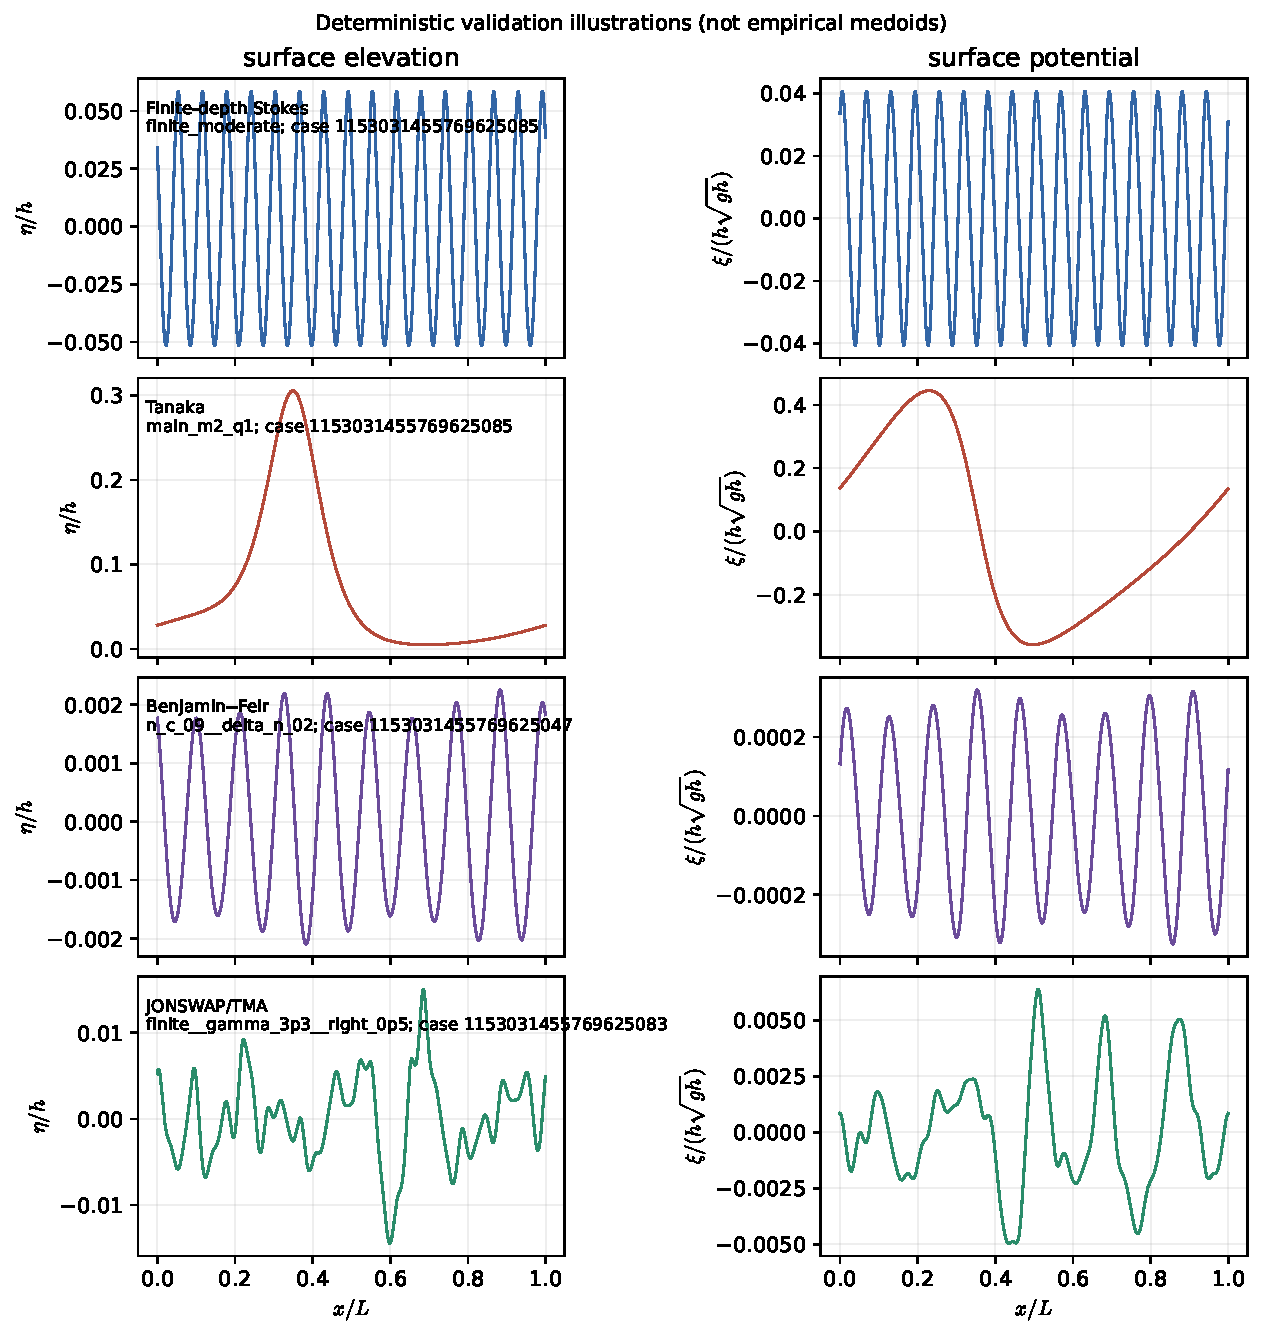
\includegraphics[width=\textwidth]{../figures/parameterized_dataset_case_examples.pdf}
  \caption{Deterministic illustrations from accepted validation cases in one
  declared central category per family, selected by the lower-median case ID;
  they are not empirical medoids.  The rows are Stokes revision~2 case
  1153031455769625085 (\texttt{finite\_moderate}), Tanaka revision~3 case
  1153031455769625085 (\texttt{main\_m2\_q1}), Benjamin--Feir revision~4
  case 1153031455769625047 (\texttt{n\_c\_09\_\_delta\_n\_02}), and
  JONSWAP/TMA revision~4 case 1153031455769625083
  (\texttt{finite\_\_gamma\_3p3\_\_right\_0p5}).  Each panel shows the
  first retained row.  The columns are the dimensionless elevation $\eta/h$
  and surface potential $\xi/(h\sqrt{gh})$, with horizontal coordinate $x/L$.}
  \label{fig:training-family-examples}
\end{figure}
\FloatBarrier

Within the JONSWAP/TMA family the design gives equal case weight to its three
depth strata.  Within the other families the listed coarse strata are likewise
balanced before seeded pseudorandom sampling within each category.  In
particular, the eleven Tanaka direction-count categories are balanced as
evenly as each finite quota permits, so their counts differ by at most one.
This gives additional aggregate weight to two- and three-crest states because
they have more direction compositions.  This is a transparent
coverage design, not a claim that all categories are equally common in nature.
If $C$ is the accepted training-case count per family selected by the learning
curve, the four-family training archive contains
$C+200C+200C+16C=417C$ stored states
before any storage-level compression.  Thus the planned learning-curve grid
$C\in\{2048,4096,8192,16384\}$ corresponds to $854{,}016$ through
$6{,}832{,}128$
training rows, while retaining $4C$ accepted training-case units.  Validation,
test, and rejected attempted cases are counted separately.
The first checkpoint uses $C=2048$ training cases per family and 1024 validation
and 1024 test cases per family.  It contains exactly
$417(2048+1024+1024)=1{,}708{,}032$ retained rows.
The production target is $C=16384$, with validation and test unchanged.  Its
7,686,144 rows are close to the 7,633,989 rows in historical v9: 52,155 more
rows, or 0.68\%.  The authenticated final view references 1,315 physical field
shards containing 94,666,557,624 measured bytes (88.165102 GiB).  Each smaller
cumulative view references an immutable source prefix rather than copying
fields.  Thus $C=2048$ is a cumulative learning-curve checkpoint, not the
completed replacement dataset.
Rejected cases are not replaced by copying nearby accepted cases; the
attempted and accepted counts are both reported.
Using a fixed number of peak periods prevents shallow categories from facing a
much longer acceptance test merely because their dimensional time scale
differs.  The historical packet \emph{training generator} stored trajectories
to final time 120.  That archive does not set either the new packet diagnostic
horizon of 20 time units or the random-sea training horizon.


\section{Attempted and accepted counts}
\label{sec:coverage}

The tables above specify attempted populations.  For every family and every
declared parameter category, report both attempted and accepted counts.  A
category with no accepted cases is not filled from another category.  Instead, generation
stops and the support or numerical method must be revised explicitly.

The population checks are computational.  The complementary Tanaka
revision-3 diagnostic chunks completed with one accepted case in each of
their eleven categories and no rejection.  Benjamin--Feir revision-4 stream
935 likewise tested one direct production-law proposal from each of its 66
categories.  The current JONSWAP/TMA constructor instead used the larger
predeclared 540-case revision-4 gate described below.

The Benjamin--Feir exact-source production gate, revision-4 stream 935,
accepted all 66 first proposals, rejected none, and retained 13,200 rows.  Its maximum implicit
stage residual was $9.999967\times10^{-9}$, maximum relative internal
Hamiltonian drift was $2.952009\times10^{-5}$, and minimum water column was
$4.960598$.

The preceding JONSWAP/TMA revision-3 stream 933 is retained only as
historical evidence for the inherited adjustment and evolution method.  It
accepted one case in every category after 29 attempts and retained 432 rows.  Its first proposals in
\texttt{finite\_\_gamma\_3p3\_\_right\_1} and
\texttt{shallow\_\_gamma\_1\_\_right\_0p5} failed during nonlinear
adjustment and retained zero rows; each canonical second proposal passed.
Over the 27 accepted cases, the maximum residual was
$9.999783\times10^{-9}$, maximum Hamiltonian drift was
$5.908800\times10^{-5}$, and minimum water column was $0.0127322$.
Thus its exact historical count was $27/29$.

The independent audit rederived all saved proposals and run specifications
and passed at
\path{outputs/nondataset_bf_revision4_jonswap_revision3_category_smoke_20260802/category_smoke_release_audit_v1.json}.
Its SHA-256 is
\par\noindent
\texttt{62fb5fe3b6be7df0d21784b1ce590c44cc484bf5fdf84ad6097fbed6f655f684}.
This artifact independently audits the Benjamin--Feir revision-4 gate and the
historical JONSWAP/TMA revision-3 gate; it does not validate the revision-4
relative-frequency constructor.  The earlier Benjamin--Feir stream-934 result
remains support-validation evidence, while stream 935 is its exact-source
revision-4 gate.  Benjamin--Feir production is complete under
\path{outputs/paper_dataset_bf_revision4_jonswap_revision3_literature_aligned_v1}.
Only its Benjamin--Feir revision-4 summaries enter the final dataset; any
JONSWAP/TMA revision-3 artifact under that historically named root is excluded.
The full source-bound completion audit is
\path{outputs/paper_dataset_bf_revision4_jonswap_revision3_literature_aligned_v1/benjamin_feir_completion_audit.json},
with SHA-256
\par\noindent
\texttt{c155b35276d0cfef6844f6b0db3e91da}\allowbreak
\texttt{3ce15579ad8b0f0ca482f44cc912753c}.
It independently verifies the current ordered 66-category taxonomy and split
quotas, reconstructed attempted/accepted/rejected counts in every category,
exact proposal replay, transaction and array hashes, accepted and rejected row
ownership, the 200 endpoint-pinned, approximately uniform selections from each
saved grid, stored depths and water columns, and the declared residual and
Hamiltonian conditions.  Two shared Python modules
changed after the run and their exact run versions were absent from the Git
history.  Their bytes are preserved as an inert audit copy, together with a
matching \texttt{SHA256SUMS} file, under
\path{reproducibility/source_snapshots/}, in the subdirectory
\path{benjamin_feir_revision4_e16773f/}.
This directory is not a current import path.  The full-dataset audit remains
the binding record for the arrays and transactions, and physically rehashes
the other 17 recorded generation sources against the current repository.  It
is distinct from the one-case-per-category gate above.

The predeclared JONSWAP/TMA revision-4 gate fixed 20 accepted cases in each
of the 27 categories before execution.  It retained 540 cases from 548
attempts; eight incomplete numerical attempts retained zero rows.  The
observed rejection rate was $1.46\%$, below the predeclared two-percent bound.
This was the completed constructor-adoption criterion, not a bulk release
threshold.
Its audited summary is
\path{outputs/jonswap_relative_band_fresh_gate_20260804/jonswap_relative_band_fresh_gate.summary.json}.
Revision-4 bulk generation uses
\path{outputs/paper_dataset_jonswap_revision4_relative_band_v1}.
The random-sea 2048-point $K=704$ versus $K=768$ sentinel remains the separate
global whole-field cutoff comparison described below.

\section{Reference evolution and whole-case acceptance}
\label{sec:acceptance}

\subsection{Discrete Zakharov flow}

The reference trajectory is the solution of a declared discrete vector field,
not merely the output of the two-stage, fourth-order Gauss--Legendre method
(GL2).  The depth $h$ remains fixed.  Let $K_{\mathrm{evol}}$ denote the
largest wavenumber retained while a trajectory is evolved.  For
$w=(\eta,\xi)$, let \(M_F\) be the evolution order assigned to family \(F\),
and define the internal DNO evaluation and the evolution-band output by
\begin{equation}
  G_{\mathrm{int},K_{\mathrm{evol}}}(\eta;h)\xi
  =\G^{N,p}_{M_F}(P_{K_{\mathrm{evol}}}\eta;h)
     (P_{K_{\mathrm{evol}}}\xi),
  \qquad
  G_{\mathrm{evol}}(\eta;h)\xi
  =P_{K_{\mathrm{evol}}}^\circ\!\left[
    G_{\mathrm{int},K_{\mathrm{evol}}}(\eta;h)\xi\right].
  \label{eq:internal-and-delivered-dno}
\end{equation}
The nonlinear product is formed with the unprojected internal output before
the evolution-band projection.  The discrete vector field is
\begin{equation}
  f_{h,K_{\mathrm{evol}}}(w)=
  \begin{bmatrix}
    G_{\mathrm{evol}}(\eta;h)\xi\\[2pt]
    P_{K_{\mathrm{evol}}}^\circ\!\left[
      -g\eta-\dfrac12\xi_x^2
      +\dfrac{\left(
        G_{\mathrm{int},K_{\mathrm{evol}}}(\eta;h)\xi
        +\eta_x\xi_x\right)^2}
             {2(1+\eta_x^2)}
    \right]
  \end{bmatrix}.
\end{equation}
Let $w_0=(\eta_0,\xi_0)$ be an admissible candidate initial state, and write
$z_0=(\eta_0,\xi_0,h)$ when the fixed depth is also needed.  The reference
ODE is
\begin{equation}
  \frac{\dd w}{\dd t}=f_{h,K_{\mathrm{evol}}}(w),
  \qquad w(0)=w_0.
  \label{eq:reference-flow}
\end{equation}
The products in the second component are evaluated on the declared dealiased
grid before projection.
We integrate this ODE with the GL2 scheme in the next subsection.
Removing the mean of $\partial_t\xi$ is precisely the time-dependent additive-potential
gauge; it preserves $\int_{\T_L}\xi\,\dd x=0$ without changing the velocity
field or the surface evolution.
The constructor sharply projects both initial fields to $|k|\leq128$.  For
Tanaka and Benjamin--Feir, this $P_{128}$ state is embedded without alteration
in the 1024-point, $K_{\mathrm{evol}}=256$ evolution space.  For JONSWAP/TMA
it is embedded in the 2048-point, $K_{\mathrm{evol}}=704$ space.  Thus every
coefficient above mode 128 initially vanishes.  The JONSWAP/TMA
adjustment defined below subsequently replaces this zero-filled state by its
full-band endpoint.  Inside every right-hand-side evaluation, both
nonlinear components are sharply projected to the relevant evolution band,
with the mean additionally removed from the $\xi$ component as in
\eqref{eq:mean-zero-band-projection}.  These projections are part of
$f_{h,K_{\mathrm{evol}}}$.

The evolution contract depends on the family and its generator revision:
\begin{center}
\begin{tabular}{@{}lccccc@{}}
  \toprule
  Family and revision & $N$ & $M_F$ & $K_{\mathrm{evol}}$ & Completed-step state map
    & Delivered band \\
  \midrule
  Tanaka revision 3 & 1024 & 6 & 256 & power-36 Hou--Li & 128 \\
  Benjamin--Feir revision 4 & 1024 & 4 & 256 & sharp $P_{256}$ & 128 \\
  JONSWAP/TMA revision 4 & 2048 & 4 & 704 & sharp $P_{704}$ & 128 \\
  \bottomrule
\end{tabular}
\end{center}
For Tanaka revision~3, after every completed GL2 step the Fourier coefficient
of each state field is multiplied by
\begin{equation}
  \sigma_k=\exp\!\left[-36\left(\frac{|k|}{256}\right)^{36}\right].
  \label{eq:tanaka-production-hou-li}
\end{equation}
The same multiplier is applied to $\eta$ and $\xi$.  Xu and Guyenne use the
power-36 Hou--Li form in their numerical method~\cite{xu2009}; the internal
cutoff $256$ is selected here by the project-specific resolution comparison
below.  For all families, the arrays presented to the dataset are
$P_{128}\eta$, $P_{128}\xi$, and the common 1024-point order-six target
$G_{\mathrm{ref}}(\eta;h)\xi$ from \eqref{eq:common-target}, evaluated from
those delivered fields.  Modes above 128 in every trajectory rollout are
numerical workspace; they are neither network inputs nor labels.
For Benjamin--Feir and JONSWAP/TMA, \(M_F=4\) determines the internal dynamics
and \(M=6\) defines the delivered learning target.

For the integrating factor, define the linear part $L_h$ and the remainder
$r_{h,K_{\mathrm{evol}}}$ by
\begin{equation}
  L_h(\eta,\xi)
  =\bigl(G_0(h)\xi,-gP_0^\perp\eta\bigr),
  \qquad
  r_{h,K_{\mathrm{evol}}}(w)
  =f_{h,K_{\mathrm{evol}}}(w)-L_hw.
  \label{eq:reference-linear-split}
\end{equation}
Benjamin--Feir starts the autonomous equation
\eqref{eq:reference-flow} directly.  The revision-4 JONSWAP/TMA path first
uses the Dommermuth nonlinear adjustment inherited from revision
3~\cite{dommermuth2000}
\begin{equation}
  \dot w
  =L_hw+A(t)r_{h,704}(w),
  \qquad
  A(t)
  =1-\exp\!\left[-\left(\frac{t}{10T_p}\right)^4\right].
  \label{eq:jonswap-nonlinear-adjustment}
\end{equation}
Dommermuth supplies the ramped-nonlinearity construction; the exponent four,
the scale $10T_p$, and the $20T_p$ handoff horizon are fixed project
settings validated below rather than unique prescriptions of that method.
For each random-sea case, this nonautonomous calculation stops at
\begin{equation}
  T_{\mathrm{adj}}
  =0.08\left\lfloor\frac{20T_p}{0.08}\right\rfloor,
  \label{eq:jonswap-adjustment-endpoint}
\end{equation}
the last saved-grid time not exceeding \(20T_p\).  Its complete
2048-point, \(K_{\mathrm{evol}}=704\) endpoint is handed to the autonomous solver without
projection to \(P_{128}\) and without rescaling either component.  The
autonomous clock is restarted at zero, \(A\) is fixed to one, and its intended
production horizon is \(16T_p\); the realized endpoint is the last saved-grid
time \(T_s\leq16T_p\).  The new Hamiltonian reference is the handoff state.
The Hamiltonian-conservation
condition below is not imposed during adjustment because
\eqref{eq:jonswap-nonlinear-adjustment} depends explicitly on time.
Finiteness, positive water depth, and convergence of every implicit stage are
still required during this adjustment.

On each nonzero Fourier mode, define
$\omega_n^2=g|k_n|\tanh(h|k_n|)$.  The linear evolution is the explicit
rotation
\begin{equation}
  \begin{bmatrix}\widehat\eta_n(t)\\ \widehat\xi_n(t)\end{bmatrix}
  =
  \begin{bmatrix}
    \cos(\omega_nt) &
      \dfrac{|k_n|\tanh(h|k_n|)}{\omega_n}\sin(\omega_nt)\\[4pt]
    -\dfrac{g}{\omega_n}\sin(\omega_nt) & \cos(\omega_nt)
  \end{bmatrix}
  \begin{bmatrix}\widehat\eta_n(0)\\ \widehat\xi_n(0)\end{bmatrix}.
  \label{eq:linear-mode-evolution}
\end{equation}
The zero modes are unchanged.  We write this linear evolution as $e^{tL_h}$.
With $v(t)=e^{-tL_h}w(t)$,
\begin{equation}
  \dot v=\widetilde F(t,v)
  :=e^{-tL_h}r_{h,K_{\mathrm{evol}}}(e^{tL_h}v).
  \label{eq:integrating-factor-field}
\end{equation}
During the JONSWAP/TMA adjustment, the right-hand side in
\eqref{eq:integrating-factor-field} is multiplied by \(A(t)\).

\subsection{Residual-controlled Gauss--Legendre stages}

The two-stage, fourth-order Gauss--Legendre coefficients are
\begin{equation}
  c_{1,2}=\frac12\mp\frac{\sqrt3}{6},\qquad
  A=\begin{bmatrix}
    \frac14&\frac14-\frac{\sqrt3}{6}\\[2pt]
    \frac14+\frac{\sqrt3}{6}&\frac14
  \end{bmatrix}.
  \label{eq:gl2-tableau}
\end{equation}
Let $t_n$ and $v_n$ be the current time and integrating-factor state, and
let $\delta_n>0$ be the step length.  Write $a_{ij}$ for the entries of the
matrix $A$ in \eqref{eq:gl2-tableau}.  The two stage values satisfy
\begin{equation}
  V_i=v_n+\delta_n\sum_{j=1}^{2}a_{ij}
       \widetilde F(t_n+c_j\delta_n,V_j),
  \qquad i=1,2.
  \label{eq:gl2-stages}
\end{equation}
After the stages converge,
\begin{equation}
  v_{n+1}=v_n+\frac{\delta_n}{2}
  \sum_{i=1}^2\widetilde F(t_n+c_i\delta_n,V_i).
  \label{eq:gl2-update}
\end{equation}

For a candidate pair $(V_1,V_2)$, define the fixed-point maps
\begin{equation}
  \Phi_i(V_1,V_2)
  =v_n+\delta_n\sum_{j=1}^{2}a_{ij}
       \widetilde F(t_n+c_j\delta_n,V_j),
  \qquad i=1,2.
  \label{eq:gl2-stage-map}
\end{equation}
Write $V_i^\eta,V_i^\xi$ and $\Phi_i^\eta,\Phi_i^\xi$ for their two
Fourier-space components, and let $\|\cdot\|_{\ell^2}$ be the Euclidean norm
of one component's Fourier coefficients.  The implemented relative stage
defect is
\begin{equation}
  R_n
  =
  \max_{\substack{i\in\{1,2\}\\u\in\{\eta,\xi\}}}
  \frac{\|\Phi_i^u-V_i^u\|_{\ell^2}}
       {\max\{\|\Phi_i^u\|_{\ell^2},
              \|V_i^u\|_{\ell^2},
              \operatorname{tiny}\}},
  \label{eq:gl2-residual}
\end{equation}
where $\operatorname{tiny}$ is the smallest positive normal number of the
working floating-point type.  Normalizing $\eta$ and $\xi$ separately avoids
adding fields with different units.  By Parseval's identity, the Fourier
normalization cancels from each ratio.

The stage tolerance $\tau_{\mathrm{GL}}$ and iteration cap are fixed in the
generator specification.  A stage is declared converged only when
$R_n\leq\tau_{\mathrm{GL}}$; otherwise its iteration ends at the declared cap
or when a nonfinite stage is detected.  Xu and Guyenne report that two to four
iterations typically achieved relative errors between $10^{-6}$ and
$10^{-8}$ in their applications~\cite{xu2009}; that observation motivates a
tolerance study, not an unchecked iteration count.  The implementation
recomputes \eqref{eq:gl2-residual} from the returned stages, freezes each
batched sample after convergence, and records finite cap exhaustion
separately from a nonfinite stage or state.  With
$\tau_{\mathrm{GL}}=10^{-8}$ and an eight-iteration cap, a four-code-path
$N=256$ smoke converged all 32 sampled steps in two updates.  The largest
residuals for Airy, finite Stokes, Tanaka, and the pre-revision BF
constructor were respectively
$9.08\times10^{-11}$, $1.10\times10^{-10}$,
$4.63\times10^{-10}$, and $2.09\times10^{-9}$.
That eight-update calculation is historical smoke evidence.  The current
paper-dataset contract permits at most four fixed-point updates per GL2 stage
for Tanaka and Benjamin--Feir and at most five for JONSWAP/TMA.  Every family
requires the same $10^{-8}$ residual.

\subsection{Method-level fixed-band resolution validation}

This validation is performed on a predeclared panel before production and
does not accept or reject individual dataset cases.  Resolution is tested by
reconstructing one physical specification, not by
interpolating one sampled array.  Fix a complete case record and re-evaluate
the same family formula with the same stored parameters on the three grids
$N_r=2^rN$, $r=0,1,2$.  Each reconstruction is performed independently in
float64.  Write $\eta_r$ and $\xi_r$ for the fields reconstructed on grid
$N_r$.  Define the dimensionless fields
\[
  U_r^{(\eta)}=\frac{\eta_r}{h},
  \qquad
  U_r^{(\xi)}=\frac{\xi_r}{h\sqrt{gh}},
\]
and write $\widehat U_{r,n}^{(\nu)}$ for the Fourier coefficient of
$U_r^{(\nu)}$, where $\nu\in\{\eta,\xi\}$.  The initial-state discrepancy is
\begin{equation}
  \Delta_{\mathrm{IC},K}
  =\max_{\nu\in\{\eta,\xi\}}\max_{0\leq r<s\leq2}
   \frac{
     \left(\sum_{|k_n|\leq K}
       |\widehat U_{r,n}^{(\nu)}-\widehat U_{s,n}^{(\nu)}|^2\right)^{1/2}}
        {\left(\sum_{|k_n|\leq K}|\widehat U_{s,n}^{(\nu)}|^2\right)^{1/2}
         +10^{-30}}.
  \label{eq:fixed-band-state-defect}
\end{equation}
On grid $N_r$, compute the target field
\begin{equation}
  G_r^\star=P_K^\circ\!\left[
    \G_M^{N_r,p}(P_K\eta_r;h)(P_K\xi_r)
  \right],
\end{equation}
set $U_r^{(G)}=G_r^\star/\sqrt{gh}$, and write
$\widehat U_{r,n}^{(G)}$ for its Fourier coefficients.  Then
\begin{equation}
  \Delta_{G,K}
  =\max_{0\leq r<s\leq2}
   \frac{
     \left(\sum_{|k_n|\leq K}
       |\widehat U_{r,n}^{(G)}-\widehat U_{s,n}^{(G)}|^2\right)^{1/2}}
        {\left(\sum_{|k_n|\leq K}|\widehat U_{s,n}^{(G)}|^2\right)^{1/2}
         +10^{-30}}.
  \label{eq:fixed-band-dno-defect}
\end{equation}
The frozen DNO threshold for this Tanaka configuration-validation panel is
$\Delta_{G,K}\leq10^{-3}$.  Both statistics are evaluated on its predeclared
cases before the Tanaka construction is frozen.  Other families use the
separately stated spatial or cutoff calculations; evidence from one family or
revision is not silently promoted to another.  A failed panel identifies an
unresolved constructor or unsupported parameter category; it does not
authorize deleting individual production rows by inspecting their shape.
Thus the expensive order-$M$ calculation is not repeated on three grids at
every stored time.

The historical Tanaka generator instead used a rowwise sign-transition rule.
If
$D_j=[G_{\mathrm{old}}(\eta;h)\xi](x_j)$ is the sampled old target, that rule
formed the cyclic forward difference
$d_j=(D_{j+1}-D_j)/\Delta x$, discarded entries below
$0.03\max_j|d_j|$, and rejected when the remaining cyclic sign sequence had
more than ten transitions.  It was useful for the old clipped-profile
constructor because a boundary seam generated oscillatory curvature, but a
resolved physical wave may also have many extrema.  In the completed Tanaka
calibration at the historical band $K=341$, all 12 matched clipped cases had
$\Delta_{G,K}\geq2.33\times10^{-2}$; the same specifications rebuilt by the
periodic constructor had $\Delta_{G,K}\leq1.10\times10^{-5}$, and four clean
controls had $\Delta_{G,K}\leq1.64\times10^{-4}$.  This supports the mechanism
without claiming that the current dataset was already filtered by the
three-grid statistic.  The tangent-Hermite construction removes the seam
mechanism, the three-grid panel checks its spatial resolution before
production, and production applies no sign-transition rejection.

The revision-3 resolution support was chosen by a separate authenticated
full-horizon calculation.  Nine one-crest specifications crossed
$\alpha\in\{0.225,0.30,0.35\}$ with
$R\in\{6,8,10\}$, where $R$ is defined in
\eqref{eq:tanaka-resolution-ratio}.  Each specification was reconstructed
once, then evolved through $T=200$ with otherwise matched internal cutoffs
$224$ and $256$.  Both calculations used float64, the multiplier
\eqref{eq:tanaka-production-hou-li} with its denominator changed to the
corresponding internal cutoff, 2,501 saved frames, and 20,000 GL2 steps.  Every
implicit stage was solved in all eighteen trajectories.

All three $R=6$ controls failed the predeclared $10^{-3}$ comparison.  Their
largest discrepancy in the delivered $G(\eta;h)\xi$ was
$9.36\times10^{-3}$.  Write $\eta_K(x,t)$ for the delivered $P_{128}$ surface
obtained with internal cutoff $K\in\{224,256\}$.  To measure the part
associated with translation, at each saved time $t$ we chose the continuous
shift $\delta(t)$ that maximized the discrete cross-correlation between
$\eta_{224}(\cdot,t)$ and $\eta_{256}(\cdot,t)$.
For
\[
  \operatorname{rms}_x[v]
  =\left(\frac1N\sum_{j=0}^{N-1}|v(x_j)|^2\right)^{1/2},
\]
the reported translation-effect statistic was
\begin{equation}
  E_{\mathrm{shift}}
  =\frac{
      \displaystyle\max_t\operatorname{rms}_x\!\left[
        \frac{\eta_{256}(\,\cdot+\delta(t),t)
                    -\eta_{256}(\,\cdot,t)}{h}
      \right]
    }{
      \displaystyle\max_t\operatorname{rms}_x\!\left[
        \frac{\eta_{256}(\,\cdot,t)}{h}
      \right]+10^{-12}
    }.
  \label{eq:tanaka-resolution-shift-effect}
\end{equation}
The largest $E_{\mathrm{shift}}$ among the $R=6$ controls was
$4.02\times10^{-3}$, and their largest hidden-band closure defect was
$2.91\times10^{-3}$.  All $R=8$ and $R=10$ cases passed.  At $R=8$, the
largest discrepancies over the three amplitudes were
\begin{equation}
  1.87\times10^{-4}\quad\hbox{in }\eta,
  \qquad 1.29\times10^{-5}\quad\hbox{in }\xi,
  \qquad 7.34\times10^{-4}\quad\hbox{in }G(\eta;h)\xi,
\end{equation}
and the largest hidden-band closure defect was $6.31\times10^{-4}$.  Thus
$R=8$ passed but used most of the $10^{-3}$ budget.  At $R=10$, the
corresponding values fell to $2.94\times10^{-5}$,
$1.62\times10^{-6}$, $1.35\times10^{-4}$, and
$1.40\times10^{-4}$.  This is a factor of about $7.1$ below the budget
and motivates the round support value $R\geq10$.

The two internal cutoffs have the same $N=1024$ physical arrays and transform
sizes in this implementation.  The exact two-times buffer
$K_{\mathrm{evol}}=256$ is therefore retained instead of $224$.  The largest
recorded Hamiltonian drift among the $R=10$ calculations was
$2.99\times10^{-8}$, but that value is only corroborating evidence from this
fixed validation panel.  It is not a production acceptance condition.  The
boundary calculation supports the conditional parameter law and the internal
resolution; it does not establish that the KdV proxy is an exact Tanaka width.

\subsection{Method-level selection of the production time step}

Two different intervals were called \texttt{dt} in earlier project notes.
Let $\Delta s$ denote the spacing between saved states and let $\delta$ denote
the actual GL2 step in \eqref{eq:gl2-stages}--\eqref{eq:gl2-update}.  If one
saved interval is divided into $m$ equal GL2 steps, then
\begin{equation}
  \delta=\frac{\Delta s}{m}.
  \label{eq:inner-gl2-step}
\end{equation}
Production uses
\begin{equation}
  \Delta s=0.08,\qquad m=8,\qquad \delta=0.01.
  \label{eq:production-gl2-step}
\end{equation}
Thus $0.08$ is a storage interval, not the step of the GL2 method.

The choice $\delta=0.01$ was made before the present dataset plan.  The May
2026 time-step study used $m=8$ while varying the saved interval through
$\Delta s\in\{0.01,0.02,0.04,0.08,0.16,0.32\}$.  In terms of the actual GL2
step, the tested values were therefore
\[
  \delta\in\{0.00125,0.0025,0.005,0.01,0.02,0.04\}.
\]
Four Tanaka cases were integrated to $T=50$.  Relative terminal elevation
differences from the $\delta=0.00125$ calculation were about $10^{-11}$,
$10^{-10}$, and $10^{-9}$ at $\delta=0.0025$, $0.005$, and $0.01$,
respectively.  The difference jumped to $6.2\times10^{-2}$ at
$\delta=0.02$.  The historical statement ``use \texttt{dt=0.08}'' therefore
selected the largest successful \emph{saved interval with eight substeps};
it selected the actual GL2 step $\delta=0.01$, not $\delta=0.08$.

Xu and Guyenne use the same GL2 step $0.01$ in their reported
calculations~\cite{xu2009}.  Their paper does not determine our saved spacing,
residual tolerance, or complete-case policy.  Those are numerical choices
for this dataset.

The step choice was checked again in July 2026 on twelve predeclared
full-horizon cases from the trajectory families.  For this method-level
validation only, each initial condition was integrated with
$\delta=0.01$ and $0.005$ and compared at common saved times.  At a saved
time $t_j$, define
\begin{align}
  Y_\delta^{(\eta)}(t_j)&=\frac{P_K\eta_\delta(t_j)}{h},&
  Y_\delta^{(\xi)}(t_j)&=\frac{P_K\xi_\delta(t_j)}{h\sqrt{gh}},&
  Y_\delta^{(G)}(t_j)&=
    \frac{G_{\mathrm{ref}}(\eta_\delta(t_j);h)\xi_\delta(t_j)}
         {\sqrt{gh}},
  \label{eq:dimensionless-delivered-fields}
\end{align}
where $(\eta_\delta,\xi_\delta)$ is the trajectory computed with GL2 step
$\delta$.  Let $\mathcal A=\{\eta,\xi,G\}$ label the three displayed fields.
For a case specification $\theta$, the validation discrepancy was
\begin{equation}
  E(\theta;\delta)
  =
  \max_{\nu\in\mathcal A}
  \frac{
    \max_j\norm{Y_{\delta/2}^{(\nu)}(t_j)
                    -Y_\delta^{(\nu)}(t_j)}_{2,L}
  }{
    \max_j\norm{Y_{\delta/2}^{(\nu)}(t_j)}_{2,L}+10^{-12}
  }.
  \label{eq:method-refinement-error}
\end{equation}
The maximum over time in the denominator prevents a temporary cancellation
of one field from producing a large relative error.  This is the historical
pre-adjustment revision-2 panel, not the revision-3 category or cutoff
comparison.  Of the twelve cases,
ten produced complete trajectories under both steps, and all ten satisfied
\[
  E(\theta;0.01)\leq1.126337\times10^{-5}.
\]
The remaining steep Tanaka and equation-(33) Benjamin--Feir cases became
incomplete at nearly the same physical times under both steps.  Halving the
step therefore neither changed an acceptance decision nor rescued either
calculation, and no $0.0025$ calculation was needed.  Together with the May
study, this panel validates the common step $\delta=0.01$.  It does not
justify repeating the half-step calculation for every production case.
On this panel the reported integration times were $4026.06$ seconds for the
$0.01$ calculations and $7798.47$ seconds for the $0.005$ calculations.  The
pair therefore used $11824.53$ seconds of integration work, whereas the
$0.01$ arm alone used $34.0\%$ of that total.  Repeating the validation pair
in production would nearly triple the measured work of the selected method.

\subsection{Historical JONSWAP/TMA spatial-cutoff calculation}

Before revision~4 changed the spectral population, the random-sea cutoff was
chosen on a predeclared shallow revision-3 sentinel.
The two independently adjusted arms used 2048 points, order four, padding
factor eight, step \(0.01\), saved spacing \(0.08\), residual tolerance
\(10^{-8}\), and an iteration cap of five.  Over the complete autonomous
history, the largest relative whole-field differences between \(K=704\) and
\(K=768\) were
\begin{equation}
  (e_\eta,e_\xi,e_{G\xi})
  =(4.64267,1.93035,7.91931)\times10^{-4}.
  \label{eq:final-jonswap-cutoff-errors}
\end{equation}
The fields were transferred by the normalized coefficients in
\eqref{eq:normalized-fourier-transfer}, and the common order-six target was
recomputed on 1024 points.  The internal order-four DNO output was not
resampled.  All three errors in \eqref{eq:final-jonswap-cutoff-errors} are
below \(10^{-3}\), while the corresponding \(K=640\) versus \(K=768\)
comparison exceeds \(10^{-3}\).  Diagnostics restricted to modes
\(96\le|k|\le128\) are about \(3\times10^{-3}\), so this calculation certifies
only the global whole-field comparison, not a bandwise bound.  Some stage
residuals lie close to \(10^{-8}\), and this is a single worst-case sentinel.
It supports the inherited $K=704$ evolution method but does not validate the
revision-4 relative-frequency population.  It therefore did not replace the
current revision-4 gate in Section~\ref{sec:coverage}.

The then-current revision-3 source was subsequently replayed from the archived
full internal \(K=704\) endpoint.  It reproduced all 289 autonomous saved
frames with maximum relative \(L^2\) errors
\((3.99\times10^{-16},4.66\times10^{-16},1.17\times10^{-15})\) in
\((\eta,\xi,G(\eta)\xi)\).  The replay was accepted, solved every stage, had
maximum residual \(9.994198\times10^{-9}\), Hamiltonian drift
\(1.831187\times10^{-5}\), minimum water column \(0.0387699\), and CPU wall
time 197.355 seconds.  This verifies that historical source and the inherited
evolution method against the archived sentinel; it does not validate the
revision-4 relative-frequency population.

\subsection{Whole-case production acceptance}

Production consequently performs one rollout per attempted trajectory case,
with $\delta=0.01$, and stores candidate states every $\Delta s=0.08$.
After the initial condition has passed its declared family support, there is
one whole-trajectory acceptance condition:
\begin{quote}
The fixed numerical method must return a complete admissible trajectory on
the requested interval $[0,T]$.
\end{quote}
Here $T$ is the horizon declared by the case.  ``Complete admissible
trajectory'' means that every scheduled GL2 step reaches $T$, every implicit
stage satisfies $R_n\leq\tau_{\mathrm{GL}}=10^{-8}$, every saved state is
finite and satisfies $h+\eta>0$ on the numerical grid, and every delivered
target $G_{\mathrm{ref}}(\eta;h)\xi$ at a saved time is finite.  Failure to
reach $T$, a nonfinite field or target, an unsolved stage, and loss of the
water-wave graph domain are diagnostic causes of this one failure condition;
they are not separate fitted filters.  If the condition fails, the complete
case is rejected and no finite prefix enters the dataset.  There is no
per-case $0.005$ comparison, discrepancy threshold, or $0.0025$ retry.

Benjamin--Feir revision-4 and JONSWAP/TMA revision-4 cases also require saved-frame
health in their full autonomous internal band.  At every autonomous saved
time \(t_j\), before projecting for delivery, let
\((N_F,K_F)=(1024,256)\) for Benjamin--Feir and
\((N_F,K_F)=(2048,704)\) for JONSWAP/TMA, set
\(\Delta x_F=2\pi/N_F\), and define
\begin{equation}
  \mathcal H_{F}(t_j)
  =\frac{\Delta x_F}{2}\sum_{\ell=0}^{N_F-1}
    \left[
      \xi_\ell(t_j)
      \bigl(G^{K_F}_4(\eta(t_j);h)\xi(t_j)\bigr)_\ell
      +g\eta_\ell(t_j)^2
    \right],
  \label{eq:production-internal-hamiltonian}
\end{equation}
where \(G^{K_F}_4\) is the order-four DNO evaluated from the complete sharp
internal state.  Let \(\varepsilon_{64}\) be the smallest positive normal
float64 number and set
\begin{equation}
  D_{\mathcal H,F}
  =\max_j
    \frac{
      |\mathcal H_F(t_j)-\mathcal H_F(0)|
    }{
      \max\{|\mathcal H_F(0)|,\varepsilon_{64}\}
    }.
  \label{eq:production-internal-hamiltonian-drift}
\end{equation}
These two families require
\(D_{\mathcal H,F}\leq10^{-3}\).  At the same dense saved frames, the
executor requires the complete internal state and
\(G^{K_F}_4(\eta;h)\xi\) to be finite and the minimum water column
\(\min_\ell\{h+\eta_\ell\}\) to be positive.  It persists the initial
Hamiltonian, maximum relative drift, minimum water column, and the state- and
DNO-finiteness indicators.  For JONSWAP/TMA, \(t=0\) and the Hamiltonian
reference in these formulas are the full-band adjustment endpoint.  No
Hamiltonian gate is applied during the nonautonomous adjustment.

There is no production gate based on sign changes, roughness, slope, extrema,
high-band energy, absolute target size, or visual appearance.  Hamiltonian
drift enters only through
\eqref{eq:production-internal-hamiltonian-drift} for the two stated
autonomous flows.

For a batch of $B$ initial conditions, the production executor advances all
$B$ cases with $\delta=0.01$.  The eight GL2 steps between consecutive
saved times are carried out inside this one batched calculation.  Random-sea
cases are grouped by their adjustment and autonomous horizons.  Each case and
its stage record are restricted to that case's declared prefix before
completeness and admissibility are decided.  Values beyond a shorter case's
horizon do not belong to that case.

\begin{figure}[ht]
  \centering
  \includegraphics[width=\textwidth]
    {../../outputs/paper_dataset_current_rejection_examples_20260726/current_rejection_examples.pdf}
  \caption{Historical illustrations of the two decision types retained in the
  current contract.  In the top row, a revision-1 finite-depth Stokes support
  redraw first proposes an amplitude with
  $\mathrm{Ur}_+=29.37>26$.  That amplitude is outside the declared Stokes
  support.  With the carrier, depth, phase, and steepness category unchanged, the
  next amplitude has $\mathrm{Ur}_+=20.34$ and is accepted.  Both displayed
  profiles are finite; the decision is the stated support inequality, not
  their appearance.  The middle and bottom rows use the $\delta=0.01$ arms of
  two July method-panel trajectories, both requested through $T=200$; they
  predate the Tanaka revision-3 and Benjamin--Feir revision-4 executors and are
  not current production attempts.  The Tanaka trajectory has its last finite saved
  state at $t=119.44$ and first failed GL2 stage at $t=119.48$.  The
  Benjamin--Feir trajectory has its last finite saved state at $t=108.72$;
  its stage at $t=108.77$ reaches eight iterations with residual
  $3.8931\times10^{-7}>10^{-8}$.  These profiles illustrate the semantics of
  whole-trajectory failure only; they do not establish the rejection of a
  current dataset case or estimate a production rejection probability.  No
  half-step calculation enters this figure or either decision.}
  \label{fig:current-rejection-examples}
\end{figure}
\FloatBarrier

Static Stokes states are not trajectories and do not use
the complete-trajectory condition.  A static case is retained only when its
declared support produces a finite state with positive water column and a
finite common target.  The three-grid, cross-family spatial audit in the
preceding subsection instead validates the constructor and common production
grid before generation; it is not a case-level filter.

The implicit stage tolerance $\tau_{\mathrm{GL}}=10^{-8}$ remains part of the
definition of the GL2 algorithm in the preceding subsection.  It specifies
when a stage equation has been solved, just as a linear-solver tolerance does;
it is not a second data-quality classifier.  Likewise, the only water-column
condition used here is the mathematical graph requirement $h+\eta>0$.  The
earlier half-depth margin $h+\eta\geq h/2$ is not part of the contract.

\subsection{Additional historical and method-panel diagnostics}

For grid index $\ell$, write $\eta_\ell=\eta(x_\ell)$ and
$\xi_\ell=\xi(x_\ell)$.  Earlier solver studies and the fixed resolution
panels monitored the following discrete energy in float64, using the
unprojected order-$M$ DNO output evaluated from the internal filtered state:
\begin{equation}
  \mathcal H_M^N(z)
  =\frac{\Delta x}{2}\sum_{\ell=0}^{N-1}
    \left[
      \xi_\ell\bigl(\G_M^{N,p}(\eta;h)\xi\bigr)_\ell
      +g\eta_\ell^2
    \right],
  \label{eq:discrete-hamiltonian}
\end{equation}
not reconstructed from the stored float32
$G_{\mathrm{ref}}(\eta;h)\xi=P_K^\circ[
\G_M^{N,p}(P_K\eta;h)(P_K\xi)]$ target.  Because the
implemented vector field includes spectral filtering and a truncated DNO,
$\mathcal H_M^N$ is not assumed to be an exact invariant of that discrete evolution;
its drift is a numerical diagnostic.
Let $z_n$ be the state after time step $n$, and set the fixed denominator
floor $\eps_{\mathcal H}=10^{-14}$.  The reported statistic is
\begin{equation}
  D_{\mathcal H}
  =\max_n
   \frac{|\mathcal H_M^N(z_n)-\mathcal H_M^N(z_0)|}
        {|\mathcal H_M^N(z_0)|+\eps_{\mathcal H} g h^2L}.
  \label{eq:hamiltonian-drift}
\end{equation}
This dimensionally floored statistic is reported on historical numerical
panels together with mass, spectra, and stage iteration counts.  It is not the
current production definition: autonomous Benjamin--Feir and JONSWAP/TMA
use the full internal-band quantity in
\eqref{eq:production-internal-hamiltonian-drift}.  Mass, spectral occupancy,
sign counts, and stage iteration counts remain diagnostics only.  Internal
Hamiltonian, state, DNO, and water-column telemetry are required production
fields only for those two current families.

\subsection{Storage after acceptance}

Every requested storage time is a GL2 step endpoint: consecutive saved times
are separated by eight steps of length $0.01$.  No temporal interpolation is
used.  Stored frames are selected only
after the numerical method has returned a complete admissible trajectory, so
a failed trajectory never contributes isolated training rows.  The
production step and saved spacing are fixed by
\eqref{eq:production-gl2-step}; they are not adjusted case by case.

\section{Reference-method and surrogate validation}
\label{sec:validation}

Xu and Guyenne~\cite{xu2009} organize validation around direct DNO tests,
truncation order, dealiasing, long-time traveling waves, invariants, and time
reversal.  The replacement generator adopts the same separation of
questions.

For two states $z=(\eta,\xi,h)$ and
$\widetilde z=(\widetilde\eta,\widetilde\xi,h)$ at the same depth, define
the dimensionless state norm
\begin{equation}
  \norm{(\eta,\xi)}_h^2
  =
  \norm{\eta/h}_{2,L}^2
  +
  \norm{\xi/(h\sqrt{gh})}_{2,L}^2,
  \label{eq:dimensionless-state-norm}
\end{equation}
where the normalized spatial norm $\norm{\cdot}_{2,L}$ is defined in
\eqref{eq:l2-conventions}.  Define
their relative state error by
\begin{equation}
  \operatorname{rel}_h(z,\widetilde z)
  =\frac{\norm{(\eta-\widetilde\eta,\xi-\widetilde\xi)}_h}
         {\norm{(\widetilde\eta,\widetilde\xi)}_h+10^{-12}}.
  \label{eq:relative-state-distance}
\end{equation}
For a validation step $\delta>0$, let $z_{\delta}$ and $z_{\delta/2}$ denote
trajectories sampled at common comparison times $t_\ell$, where $\ell$
indexes those times.  Define the method-level temporal defect by
\begin{equation}
  E_t(\delta)
  =\max_\ell \operatorname{rel}_h\!\left(
    z_{\delta}(t_\ell),z_{\delta/2}(t_\ell)\right).
  \label{eq:temporal-refinement-defect}
\end{equation}
For a traveling profile, let $\sigma\in[0,L)$ denote a horizontal translation
and define
\begin{equation}
  E_{\mathrm{shape}}(t)
  =\min_{\sigma\in[0,L)}
   \frac{\norm{\eta(\cdot,t)-\eta(\cdot-\sigma,0)}_{2,L}}
        {\norm{\eta(\cdot,0)}_{2,L}+10^{-12}},
  \label{eq:translation-aligned-shape-error}
\end{equation}
and obtain the numerical displacement from the minimizing $\sigma$.
Starting from $z_0$, integrate to time $T$ and call the result
$z_{\mathrm f}$.  Starting from $z_{\mathrm f}$, use the same step
lengths in reverse order with negative sign and call the returned state
$z_{\mathrm b}$.  The forward--backward defect is
\begin{equation}
  E_{\mathrm{rev}}(T)
  =\operatorname{rel}_h(z_{\mathrm b},z_0).
  \label{eq:reversibility-defect}
\end{equation}
Thus the forward and backward calculations use exactly the same step lengths.

\begin{table}[ht]
  \centering
  \caption{Validation objects, measured quantities, and decision roles.}
  \label{tab:validation-roles}
  \small
  \begin{tabularx}{\textwidth}{
    @{}>{\raggedright\arraybackslash}p{0.20\textwidth}
       >{\raggedright\arraybackslash}X
       >{\raggedright\arraybackslash}p{0.25\textwidth}@{}}
    \toprule
    Panel & Quantity reported & Role \\
    \midrule
    Manufactured DNO
      & Exact-DNO error, discrete-target error, learned-target error, and
        end-to-end error as defined in Appendix~\ref{sec:manufactured}.
      & Selects the discrete reference configuration, not network weights. \\
    Three-grid construction
      & $\Delta_{\mathrm{IC},K}$ and $\Delta_{G,K}$ from
        \eqref{eq:fixed-band-state-defect}--\eqref{eq:fixed-band-dno-defect}.
      & Required before production; validates each constructor and the common
        spatial configuration. \\
    Time-step study
      & $E_t(\delta)$, maximum stage residual, and $D_{\mathcal H}$.
      & Required before production; selects one common GL2 step.  It is a
        method-level panel, not a calculation repeated for each dataset case. \\
    Traveling Stokes/Tanaka
      & $E_{\mathrm{shape}}(t)$, displacement divided by $t$, mass,
        \eqref{eq:hamiltonian-drift}, and $E_{\mathrm{rev}}(T)$.
      & Validates long-time propagation of the reference method. \\
    Benjamin--Feir
      & Modal amplitudes $2|\widehat\eta_n(t)|$ at the carrier and sidebands,
        recurrence error, $D_{\mathcal H}$, and high-band energy.
      & Validates modulation dynamics; growth alone is not labeled breaking. \\
    Airy
      & Flat-surface identity and cubic small-amplitude remainder scaling.
      & Post-freeze architecture verification only. \\
    Sparse Fourier
      & One-step DNO error and complete rollout error; nonfinite rollouts
        count as infinite error.
      & Development cases select only the dataset; final cases only report. \\
    Support sensitivity
      & Cellwise attempted/accepted counts under predeclared neighboring
        family-support bounds.
      & Tests whether a declared support bound removes a difficult parameter
        category; it does not alter the fixed production step. \\
    \bottomrule
  \end{tabularx}
\end{table}

Every appearance of $D_{\mathcal H}$ in
Table~\ref{tab:validation-roles} refers to the historical or fixed
method-level diagnostic defined in \eqref{eq:hamiltonian-drift}; it is not a
row, case, or trajectory acceptance condition.

Successive-$M$ differences on general states are called order sensitivity,
not convergence to the physical DNO, unless an independent boundary-integral
or conformal reference is supplied.  This qualification matters because
Xu--Guyenne report an amplitude- and resolution-dependent optimal order:
larger $M$ need not reduce error once the recursion is ill-conditioned.

The completed three-grid Tanaka study remains useful evidence that periodic
wrapping removes the old clipped-profile defect.  It does not by itself
validate the four training families, the three diagnostic suites, the time
integrator, or the choice $M=6$.

\section{Temporal sampling, splitting, and normalization}
\label{sec:splitting}

Temporal selection is performed only after the fixed-step calculation has
returned a complete admissible trajectory.  Tanaka is evaluated on the dense
time grid
\begin{equation}
  t_j=0.08j,\qquad j=0,\ldots,2500,
  \label{eq:adaptive-dense-times}
\end{equation}
and 200 times are retained for each case.  The internal GL2 step
is $0.01$; $0.08$ is the spacing of the candidate storage grid.

For Tanaka, define the discrete surface-gradient energy and its activity by
\begin{equation}
  S_{\mathrm T,j}=\sum_{\ell=0}^{N-1}
    |\partial_x\eta(x_\ell,t_j)|^2,
  \qquad
  A_{\mathrm T,j}
  =\frac{|\delta S_{\mathrm T,j}|}{S_{\mathrm T,j}+10^{-12}}.
  \label{eq:tanaka-time-activity}
\end{equation}
Here
\[
  \delta S_0=S_1-S_0,\qquad
  \delta S_j=\frac{S_{j+1}-S_{j-1}}2\ (1\leq j\leq2499),\qquad
  \delta S_{2500}=S_{2500}-S_{2499}.
\]
The derivative $\partial_x\eta$ is computed by the Fourier multiplier
$ik_n$ on the common grid.  Thus Tanaka receives extra samples
when the spatial surface derivative changes rapidly during crest interaction.

Convolve the nonnegative Tanaka activity values with a normalized discrete
Gaussian, extending the endpoint values outside the time interval.  The
Gaussian standard deviation is 50 candidate-time steps, and its support is
truncated at three standard deviations, rounded upward to an integer number
of time indices.  Call the smoothed values $\widetilde A_{\mathrm T,j}$ and
define
\begin{equation}
  p_{\mathrm T,j}=\frac{1-\alpha_{\mathrm T}}{2501}
    +\alpha_{\mathrm T}\frac{\widetilde A_{\mathrm T,j}}
      {\sum_{r=0}^{2500}\widetilde A_{\mathrm T,r}},
  \qquad \alpha_{\mathrm T}=0.5.
  \label{eq:adaptive-time-density}
\end{equation}
If the smoothed activity vanishes identically, its normalized term is replaced
by the uniform distribution.  The 200 retained indices are the deterministic
inverse-CDF locations of the midpoint quantiles
$(\ell+1/2)/200$, $\ell=0,\ldots,199$.  The first and last candidate times are
included, repeated indices are advanced to the next unused index, and all
selected indices and activity parameters are stored with the case.  This rule
depends only on the accepted reference trajectory, never on model error.

For a Benjamin--Feir trajectory, let
$J_{\mathrm{BF}}=T_{\mathrm{BF}}/0.08$, where $T_{\mathrm{BF}}$ is defined in
\eqref{eq:bf-carrier-period-horizon}.  Retain the 200 saved-grid indices
\begin{equation}
  j_\ell
  =\left\lfloor\frac{\ell J_{\mathrm{BF}}}{199}+\frac12\right\rfloor,
  \qquad \ell=0,\ldots,199.
  \label{eq:bf-uniform-time-selection}
\end{equation}
These indices are approximately uniform in time and include both endpoints.
The Benjamin--Feir storage rule therefore introduces no additional event
score.

For a random-sea trajectory, let
\[
  T_{\mathrm{hor}}=16\frac{2\pi}{\omega_p},
  \qquad
  T_s=0.08\left\lfloor\frac{T_{\mathrm{hor}}}{0.08}\right\rfloor,
  \qquad
  J_s=\frac{T_s}{0.08}.
\]
It retains the saved-grid indices
\[
  j_\ell=\left\lfloor\frac{\ell J_s}{15}+\frac12\right\rfloor,
  \qquad
  t_\ell=0.08j_\ell,
  \qquad \ell=0,\ldots,15.
\]
Thus the integration ends at the last saved-grid point not exceeding sixteen
peak periods, and the retained endpoints are $0$ and $T_s$.  For
JONSWAP/TMA, this \(t=0\) is the complete 2048-point, \(K=704\) adjustment endpoint and
the start of the autonomous clock, not the initial linear random sea.  Static
Stokes cases retain only $t=0$, with phase already contained in the case
record.

Random-sea cases in one numerical batch can have different values of $T_s$.
The single production batch is advanced to the longest required saved-grid
endpoint in the batch, but each case's fields and GL2 stage record are cropped
to its own declared prefix before completeness and admissibility are decided.
Hence values after a shorter case's horizon cannot affect its acceptance.  A
regression test obtains the same decision, retained fields, and prefix stage
record in serial and batched runs even when post-horizon values are
deliberately made nonfinite.  Batch size is recorded per launch.  The completed
Tanaka revision-3 gate used batch sizes six and five for its complementary
chunks.  The two excluded historical 1024-case training shards used batch
size 256; this changed transaction granularity, not the population law.

Training, validation, and test cases come from three disjoint tagged
PCG64 construction streams.  Their root seeds are respectively
2026072210, 2026072204, and 2026072205.
Every attempted case stores its root seed, stream identifier, and realized
parameters.  Let $s$ be the split root, let $f$ identify the physical family,
let $v$ identify the generator revision, let $r$ be the stream identifier,
and let $a$ be the attempted-case index.  Every family initializes its
per-case PCG64 stream from the five integer words $(s,f,v,r,a)$.  Thus replay
of one attempted case reproduces its complete specification without depending
on the number of earlier accepted cases.  Split membership is therefore fixed
when the attempted case specification is written, before integration or time
selection; it is not assigned from the resulting trajectory.  The training
stream continues until it has the post-acceptance count $C$ per family selected
by the learning curve.  The validation and test streams each contain 1,024
accepted cases per family, balanced over the same parameter categories to
within one case.  Every
rejected attempt remains attached to its original split manifest.
A nested training chunk is never enlarged in place.  The successive
$(C_0,A)$ pairs, where $C_0$ is the preceding cumulative count and $A$ is the
new count per family, are
\[
  (0,2048),\ (2048,2048),\ (4096,4096),\
  (8192,8192).
\]
They use distinct stream identifiers $0,1,2,3$ and the category increments in
\eqref{eq:additive-cell-quota}.  Validation and test each use one fixed,
non-nested chunk.
A requested count in one family--split category is never filled by copying or
silently drawing from another category.  In the static Stokes generator, one
candidate fixes the mode, depth, phase, and steepness category and permits at most
1000 amplitude redraws within that same category.  The sampler record contains
every rejected amplitude and its $\mathrm{Ur}_+$ value, followed by the
accepted amplitude on success.  If all 1000 redraws are exhausted, the sampler
raises with the complete strict record.  The implemented static executor
stores that record as a zero-row out-of-support attempt and schedules a
replacement in the same category.  It is not a fatal batch error.  An
unclassified error propagates without being relabeled; only the trajectory
executor's explicit fatal exception writes a terminal failure record.
This internal amplitude-redraw limit does not consume additional outer
attempts.  The replacement case does consume the next durable attempt under
\eqref{eq:cell-attempt-ceiling}.

No two temporal snapshots from the same case can appear in different
subsets.  This removes exact temporal-sibling leakage; it does not imply that
nearby parameter draws are statistically independent.

The loader implements the case-balanced rule stated in
Section~\ref{sec:dataset-design}: it selects exactly one stored time from
every accepted training case in every epoch and batches those selected rows.
The validation time for each case is fixed deterministically.  A different
number of stored times requires a separate learning-curve comparison; it is
not chosen from rollout failures.

Let $\mathcal I_{\mathrm{train}}$ denote all stored rows from accepted
training cases.  For row $i\in\mathcal I_{\mathrm{train}}$, let $\eta_i$ and
$\xi_i$ be its two input fields, let $h_i$ be its depth, and let
$G_i^\star=G_{\mathrm{ref}}(\eta_i;h_i)\xi_i$ be its target from
\eqref{eq:common-target}.  The network retains the scale normalization used by
the strongest current checkpoint, but estimates it on this set only:
\begin{equation}
  s_\eta=\max_{i\in\mathcal I_{\mathrm{train}},x}|\eta_i(x)|,
  \qquad
  s_\xi=\max_{i\in\mathcal I_{\mathrm{train}},x}|\xi_i(x)|,
  \qquad
  s_G=\max_{i\in\mathcal I_{\mathrm{train}},x}|G_i^\star(x)|.
  \label{eq:training-scales}
\end{equation}
Let $h_\star=L/(2\pi)$ be the fixed reference length.  For one row, write
$(\eta,\xi,h,G^\star)$ for its two input fields, depth, and target.  The
network receives
\begin{equation}
  \widetilde\eta=\eta/s_\eta,\qquad
  \widetilde\xi=\xi/s_\xi,\qquad
  d_h=\log\!\left(\frac{h}{h_\star}\right),\qquad
  \widetilde G^\star=G^\star/s_G.
  \label{eq:network-normalization}
\end{equation}
Hence $d_h$ is
dimensionless and is unchanged by the period rescaling in
Appendix~\ref{app:dno-rescaling}; on the production domain $L=2\pi$ it has
the same numerical value as the existing input $\log h$.
The authenticated training-only values are
$s_\eta=0.15583430230617523$,
$s_\xi=0.09394174814224243$, and
$s_G=0.12198150902986526$, computed from 6,832,128 rows.  The release audit
verifies all three before training.  The current loader nevertheless
uses one as a defensive fallback if a nonpositive scale reaches it; the
writeup does not count that fallback as validation of a malformed dataset.
Their statistics fingerprint is
\texttt{4e8ec96947bc05ce}\allowbreak
\texttt{e3b375467499b0ae}\allowbreak
\texttt{00a7814f99826140}\allowbreak
\texttt{84efd859efe7c3b8}.
No per-family, per-mode, validation, or diagnostic statistic enters
\eqref{eq:training-scales}.  The cached scales are bound to the checked
identity of the assembled dataset.
Reports include both the number of case units and the number of stored
snapshots.  Dataset size is selected by a learning curve in accepted case
count, rather than by reproducing the \texttt{v9} snapshot count by default.
The Airy, manufactured, and sparse diagnostic cases are absent from all three
training subsets and from the training-scale calculation.  If a diagnostic
result motivates a redesign, the final paper reports a fresh, case-disjoint
diagnostic draw after the revised model is frozen.

At $C$ accepted training cases per family, the case-balanced loader presents
$4C$ samples per epoch.  With global batch size 1024, comparisons at a fixed
epoch count would therefore give larger corpora more optimizer updates.  The
learning curve instead uses 10,240 optimizer updates:
\begin{center}
\begin{tabular}{@{}rrr@{}}
  \toprule
  $C$ & Steps per epoch & Epochs for 10,240 updates \\
  \midrule
  2,048  & 8   & 1,280 \\
  4,096  & 16  & 640 \\
  8,192  & 32  & 320 \\
  16,384 & 64  & 160 \\
  \bottomrule
\end{tabular}
\end{center}
The learning-rate schedule is a function of optimizer step, not epoch.
Checkpoints are compared at the same predeclared update numbers; the number
of epoch boundaries is not allowed to give the smaller dataset more
checkpoint-selection opportunities.  Test errors are first aggregated by
case within each family and then with equal weight across the four families.
A single statistic weighted by the 1, 200, 200, and 16 stored rows per case
is not a paper-level four-family result.

\section{Execution plan}
\label{sec:execution}

The target, four population laws, spatial window, reference integrator,
complete-trajectory condition, storage rule, and bounded quota mechanism are
frozen.  Before the production executor was simplified to one time step, an
exact-contract four-family smoke used run-specification schema 1 and computed
the $0.01/0.005$ validation pair:
\begin{center}
\small
\begin{tabular}{@{}lrrrr@{}}
  \toprule
  Family & Accepted & Rows & Pair discrepancy & Wall time (s) \\
  \midrule
  Stokes & 1 & 1   & ---                       & 3.782 \\
  Tanaka & 1 & 200 & $3.1953\times10^{-8}$     & 5,555.35 \\
  Benjamin--Feir & 1 & 200 & $3.7058\times10^{-8}$ & 5,561.11 \\
  JONSWAP/TMA & 1 & 16 & $7.6600\times10^{-7}$  & 835.19 \\
  \bottomrule
\end{tabular}
\end{center}
The four cases assembled into one checked dataset view containing 417 finite
rows on 1024 points, and the loader selected one time from each case.  The
pair discrepancies are historical method-validation evidence, and the
recorded wall times include work that production no longer performs.  These
run-spec-schema-1 artifacts predate both the bounded scheduler and Tanaka
revision~3.  They deliberately cannot resume as a current production run.

Generator revision is a family-specific identity, not one global integer.
The present revision map is
\begin{equation}
  (v_{\mathrm{Stokes}},v_{\mathrm{Tanaka}},v_{\mathrm{BF}},v_{\mathrm{sea}})
  =(2,3,4,4).
  \label{eq:paper-family-revisions}
\end{equation}
Here $v_{\mathrm{BF}}$ is the Benjamin--Feir revision and $v_{\mathrm{sea}}$
is the JONSWAP/TMA revision.  Revision-1 smokes and all superseded revision-2
trajectory artifacts remain historical constructor, transaction, or
method-selection evidence.  They cannot be resumed into an output directory
with a different family revision or counted toward its quota.  A combined dataset view requires
exactly one revision per family.  Within each
$(\text{family},\text{revision})$ pair it requires one numerical execution
identity and one generator-source identity; it does not require the filtered
Tanaka order-six execution record to equal the sharp Benjamin--Feir or
JONSWAP/TMA order-four records.

Current revision-2 Stokes evidence includes one exact case from each of
the four Stokes categories.  All four were accepted, their quality-decision
masks were zero, and the complete calculation took $4.6875$ seconds.  Its
production splits are also complete at 16384 training, 1024 validation, and
1024 test cases; they are preserved.  The
older reduced real-GL2 transactions from the trajectory families check
historical software wiring only.  For Tanaka revision~3, the full-horizon
boundary calculation in Section~\ref{sec:acceptance} has frozen the
amplitude-first $R\geq10$ support and $K_{\mathrm{evol}}=256$ Hou--Li
execution contract.  Before this Tanaka category pilot, 50 focused
contract/manifest tests, 212 generator tests, and 102 script tests passed.

At 16:09 on 31 July 2026, the exact Tanaka revision-3 production pilot was
launched in two complementary chunks.  The first requests category codes
0--5 and the second requests codes 6--10, so together they request one case
from every one of the eleven Tanaka categories.  Their durable batch-zero
proposals were written before construction.  Both chunks use
\eqref{eq:tanaka-conditional-depth-law},
$K_{\mathrm{evol}}=256$, \eqref{eq:tanaka-production-hou-li}, delivered
$P_{128}$ rows and labels, GL2 step $0.01$, and only the construction-domain
and complete-trajectory decisions stated above.  Both chunks completed.  The
first recorded 6 accepted, 6 attempted, and 0 rejected cases; the second
recorded 5 accepted, 5 attempted, and 0 rejected cases.  Together they cover
cell codes 0--10 exactly once and contain eleven distinct case identities.
Every trajectory reaches $T=200$, has 2501 saved frames, retains 200 selected
rows, keeps a positive water column, and solves every GL2 step.  The maximum
relative stage residual over all eleven cases is
$9.997\times10^{-9}$.  Every case has required, evaluated, and failed quality
masks respectively equal to 768, 791, and 0.

The configuration fingerprints of the two completed pilot chunks are,
respectively,
\begin{center}
\footnotesize
\begin{tabular}{@{}l@{}}
\texttt{3a107cc1e4a711f48c35a0f1995f484552b658f0f926ee324e487cee940fbda8}\\
\texttt{c089df6be04f25c4c59794f0e34599ee457e0db076e807834608fed1c5c62b9f}.
\end{tabular}
\end{center}
Their summary-file SHA-256 digests are, in the same order,
\begin{center}
\footnotesize
\begin{tabular}{@{}l@{}}
\texttt{075dd7c30d325fc5034b6ee9350949a99317ae22e1656c4597f93d4de4cfe164}\\
\texttt{cd24c7a801150667b5872332baa38353865f4ae04349c9cfd75ae4f1fc87e7df}.
\end{tabular}
\end{center}
The two summaries carry identical numerical, dependency, and source-hash
tables, and those hashes match the frozen files.  The measured wall times were
1493.31 seconds for the six-case chunk and 2931.72 seconds for the five-case
chunk.  Their 2200 validation-tagged pilot rows remain outside the final
dataset.

This result freezes Tanaka revision~3 as generation-ready with the conditional
$R\geq10$ support, one sharp $P_{128}$ initial projection, a zero-filled
$K_{\mathrm{evol}}=256$ workspace, the power-36 Hou--Li multiplier after every
completed step, and delivered $P_{128}$ rows and labels.  It adds no
Hamiltonian, sign-count, slope, roughness, or spectral rejection rule.

At 17:02 on 31 July 2026, two complementary 1024-case Tanaka training chunks
were launched for cumulative accepted intervals $0{:}1024$ and
$1024{:}2048$, with separate streams, batch size 256, and configuration
fingerprints
\begin{center}
\footnotesize
\begin{tabular}{@{}l@{}}
\texttt{d4b38dea49ade42f0251aeb993c935155cd07a516475a2d922c48226ca4973c1}\\
\texttt{ccd5968fcb936501245e5b1858282b953fdfee9e65d027e66bc323783d38da3f}.
\end{tabular}
\end{center}
They use the frozen revision-3 contract above.  Both training chunks and the
corresponding 1024-case validation and test chunks completed, with all 4096
attempts accepted and 200 rows retained per case.  These artifacts are now
historical and are excluded from the paper dataset.

The old solitary-wave solve had an effective component-amplitude floor of
$9.9478\times10^{-4}$.  Exactly 64 of the 4096 cases request one component
below this floor; the worst is inflated by $41.27\times$ after the complete
periodic construction and projection.  The old trajectory rows are therefore
excluded.  The corrected population remains revision 3 but draws a fresh
deterministic population with 16384 training cases and 1024 cases in each of
validation and test; it does not reuse the historical random specifications.

The source-authenticated release is complete.  Stokes retained 18432 cases
from 18432 attempts and stored 18432 rows; corrected Tanaka retained
18432/18432 and stored 3686400 rows; Benjamin--Feir retained 18432/18455 and
stored 3686400 rows; and JONSWAP/TMA retained 18432/18726 and stored 294912
rows.  The aggregate is 73728 accepted cases from 74045 attempts, 317
zero-row rejections, and 7686144 rows.  The exact cumulative combined-summary
SHA-256 identities at 2048, 4096, 8192, and 16384 training cases per family
are
\texttt{2265cb71270accb3}\allowbreak
\texttt{f6d9103e90433b664}\allowbreak
\texttt{ca813989dfab6340}\allowbreak
\texttt{3d8612af22d28c3},
\texttt{7feb018ee4d94eab}\allowbreak
\texttt{10278917c1452620}\allowbreak
\texttt{26cccab6169eaaa2}\allowbreak
\texttt{d8877f7c7b28c9da},
\texttt{43b1eb91198e724c}\allowbreak
\texttt{6f32b871c2d0efd0}\allowbreak
\texttt{d8355533789919df}\allowbreak
\texttt{5897ad588e7e85f6},
and
\texttt{32f764cf865c9089}\allowbreak
\texttt{2ee0329e48fe992c}\allowbreak
\texttt{bc24df2707e05fd1}\allowbreak
\texttt{af2ee9cd2b84307c}.
The immutable document handoff reports the exact attempted, accepted, and
rejected marginal for every declared family, split, and parameter category,
thereby closing the reporting contract above.  Its SHA-256 identity is
\begin{center}
\small
\texttt{b21830cf56f9c17a1ee165624c71fdc0e286727747d364330fbace19e5ef6053}.
\end{center}
No reported model has been trained on this dataset.  The remaining empirical
work is:

\begin{enumerate}
  \item \textbf{Run the complete nested learning curve.}
        Extend the training split additively to
        \[
          C\in\{2048,4096,8192,16384\}
        \]
        accepted cases per family while keeping validation and test fixed.
        The final point contains 7,686,144 retained rows, comparable to
        historical v9's 7,633,989 snapshots.
        Train two seeds at every $C$ with the same architecture, optimizer,
        and 10,240-update schedule.  Compare final checkpoints at that common
        update count.  Report every point rather than stopping at an undefined
        ``material improvement'' threshold.

  \item \textbf{Test shallow mixed-mode coverage.}
        Evaluate every learning-curve endpoint on the 11 historical
        shallow-steep cases and the frozen sparse development panel.  The
        existing checkpoint C27, trained on all \texttt{v9} sources, is an
        external performance baseline, not a matched ablation.  Measure
        relative terminal elevation error and assign infinite error to every
        nonfinite rollout.  Report the median, 95th percentile, nonfinite
        count, and counts above $0.25$, $0.50$, $0.75$, and $1$.  A failure
        motivates a separately versioned population revision; it does not
        change this frozen dataset after results are seen.

  \item \textbf{Freeze and test once.}
        After all models and checkpoints are fixed, evaluate the untouched
        training-family test cases, Airy panel, manufactured-DNO panel, and
        final sparse panel.  Report errors by case within family and then
        weight the four family summaries equally.  Any later design change
        requires a new final sparse draw.
\end{enumerate}

\section{Claims this plan does and does not support}

The completed dataset supports the following statements:
\begin{itemize}
  \item every attempted initial condition is reproducible from a complete,
        finite-dimensional case specification and one common configuration;
  \item every training label uses the same discrete operator convention;
  \item training, validation, and test rows come from disjoint cases;
  \item no Airy, manufactured-harmonic, or sparse-Fourier diagnostic row
        contributes to optimization or empirical normalization;
  \item every saved state of an accepted reference trajectory remains in the
        water-wave graph domain, and the trajectory is complete under the
        declared fixed GL2 method; and
  \item the declared four-family depth, nonlinearity, and spectral coverage is
        reported in physical dimensionless variables.
\end{itemize}

It does not, without further analysis, support the stronger statements that
the selected $G_M$ equals the physical DNO, that Hamiltonian conservation proves trajectory
accuracy, that JONSWAP spans every physically relevant sea, or that a
trajectory rejected by this numerical method is physically impossible.
Success on the four training families also does not establish arbitrary
mixed-mode generalization or accuracy below the declared shallow-TMA depth;
those remain empirical questions measured by the diagnostic suites.  The
existing C27 result cannot answer the dataset-ablation question because C27
was trained on all \texttt{v9} sources.  The order, grid, timestep, benchmark,
and new-dataset retraining studies are included precisely to keep those
questions separate.

\appendix

\section{Audit of the current \texttt{v9} archive}
\label{sec:v9}

The archive \texttt{combined\_dataset\_v9.npz} contains $7{,}633{,}989$
snapshots on $N=1024$ points over $L=2\pi$.  Its six construction categories
are Gaussian seas (460,740 rows), manufactured single modes (500,000),
fifth-order Stokes states (1,000,000), Tanaka-profile states (2,200,000),
Benjamin--Feir states (2,033,249), and sparse Fourier packets (1,440,000).
The suffixes \texttt{g0}, \texttt{g1}, and \texttt{modal} name generator runs,
not different initial-condition families or DNO orders.

The archive remains a valuable empirical baseline.  It was assembled from
generators with different row counts, filtering rules, and target
conventions.  The relevant distinctions are summarized in
Table~\ref{tab:v9-defects}.

\begin{table}[ht]
  \centering
  \caption{Why the flat \texttt{v9} archive does not define the replacement
  paper dataset.}
  \label{tab:v9-defects}
  \small
  \begin{tabularx}{\textwidth}{
    @{}>{\raggedright\arraybackslash}p{0.19\textwidth}
       >{\raggedright\arraybackslash}X
       >{\raggedright\arraybackslash}p{0.29\textwidth}@{}}
    \toprule
    Object & Current archive & Replacement rule \\
    \midrule
    Sampling rule
      & Source-dependent numbers of stored times make snapshot weight differ
        from case weight.
      & In every epoch select one stored time from every accepted case, then
        batch those selected rows. \\
    Discrete target
      & Static sources retain the direct order-six output, whereas rollout
        sources are projected to $|k|\leq128$.
      & Use \eqref{eq:common-target} for every row. \\
    Acceptance
      & Early sources were filtered rowwise; later sources used
        source-specific whole-case Hamiltonian tests.
      & Use declared support for static Stokes states and one complete
        fixed-step numerical-path condition for each trajectory family.
        Benjamin--Feir revision~4 and autonomous JONSWAP/TMA revision~4 additionally
        require the declared internal Hamiltonian bound
        \eqref{eq:production-internal-hamiltonian-drift}. \\
    Reconstructibility
      & Some phase arrays and case fields were not stored, and no stage
        residual was recorded.
      & Store every parameter and test the residual
        \eqref{eq:gl2-residual}. \\
    Statistical split
      & A rowwise split can place temporal siblings in different subsets;
        normalization used the complete archive.
      & Split by attempted case and fit scales on accepted training cases. \\
    Support changes
      & Some failed parameter combinations were replaced by hand, for example
        one Benjamin--Feir mode pair.
      & Declare support first; record rejection without changing parameters. \\
    \bottomrule
  \end{tabularx}
\end{table}

Table~\ref{tab:v9-supports} records the historical parameter envelopes needed
for the direct comparison.  These are support bounds, not empirical
quantiles, and independent dimensional draws did not induce uniform density
in the dimensionless coordinates used below.  Here $H_s$ is significant wave
height, $k$ is wavenumber, $k_p$ is peak wavenumber, $k_c$ is carrier
wavenumber, $b$ is spectral bandwidth, and $n$, $n_c$, and $n_j$ are Fourier
mode indices.  The symbols $a$ and $a_j$ are wave amplitudes, $\Delta n$ is
sideband separation, and $\rho_\pm$ are sideband-to-carrier amplitude ratios.

\begin{table}[ht]
  \centering
  \caption{Historical support envelopes retained for comparison.}
  \label{tab:v9-supports}
  \small
  \begin{tabularx}{\textwidth}{
    @{}>{\raggedright\arraybackslash}p{0.18\textwidth}
       >{\raggedright\arraybackslash}X@{}}
    \toprule
    Construction & Declared support in \texttt{v9} \\
    \midrule
    Gaussian sea
      & $H_s\in[0.005,0.03]$, $k_p\in[2,12]$, bandwidth
        $b\in[1.5,5]$; $h\in[0.1,1.5]$ or $h\in[5,25]$. \\
    Manufactured mode
      & $n\in\{1,\ldots,20\}$, $h\in[0.02,1.5]$,
        $kh\in[0.02,20]$, and $0.005\leq ka\leq0.15$, subject to
        $a\in[10^{-4},0.011494]$. \\
    Stokes
      & Deep: $n\in\{1,\ldots,20\}$, $h\in[4,50]$.
        Finite: $n\in\{14,\ldots,26\}$, $h\in[0.02,1.5]$,
        $kh\in[0.5,5]$.  Both impose $ka\leq0.15$. \\
    Tanaka
      & Main: $h\in[0.01,0.30]$, one to three crests, total
        $\sum_j a_j/h\in[0.10,0.35]$.  Steep: $h\in[0.20,0.35]$,
        one crest, $a/h\in[0.25,0.45]$. \\
    Benjamin--Feir
      & $h\in[0.5,4]$, $n_c\in\{4,\ldots,20\}$,
        $k_ca\in[0.05,0.13]$, $\Delta n\in\{2,3,4\}$, and
        $\rho_\pm\in[0.05,0.20]$. \\
    Sparse Fourier
      & One to five modes, $h\in[0.005,0.5]$,
        $kh\in[0.2,1.5]$, total $a/h\in[0.03,0.25]$, and
        $\sum_j n_ja_j\leq0.15$. \\
    \bottomrule
  \end{tabularx}
\end{table}

Two historical formulas matter for interpreting the redesign.  First, the
old sea uses the following Gaussian elevation spectrum rather than the
JONSWAP/TMA construction in Section~\ref{sec:jonswap}:
\begin{equation}
  S_{\mathrm{old}}(k;k_p,b)
  =\exp\!\left[-\frac{(|k|-k_p)^2}{2(k_p/b)^2}\right].
  \label{eq:old-gaussian-spectrum}
\end{equation}
Second, the source archived as \emph{linear} is a manufactured harmonic
trace.  For wavenumber $k$, amplitude $a$, phase $\phi$, and direction sign
$s\in\{-1,1\}$, set $\vartheta=kx+\phi$ and
$\omega^2=gk\tanh(kh)$.  Then
\begin{align}
  \eta(x)&=a\cos\vartheta,\\
  \xi(x)&=s\,\frac{ag}{\omega}
    \frac{\cosh(k(h+\eta(x)))}{\cosh(kh)}\sin\vartheta.
  \label{eq:old-manufactured-xi}
\end{align}
The nonlinear dependence on $\eta$ makes this an exact manufactured
boundary trace, not a separate physical linear-wave family.

The historical depth union is approximately $0.005\leq h\leq50$.  This is
not automatically the support of the replacement dataset.  The four-family
design reaches $h\simeq0.0083$ through its shallow random-sea stratum and
$h=50$ through
Stokes; the smaller-depth interval remains diagnostic unless a separate
resolution study admits it.  The full source-by-source audit is therefore
evidence for the redesign, not the main definition of it.


\section{Diagnostic specifications and separation from training}
\label{sec:diagnostic-specifications}

The three diagnostic suites are Airy, exact manufactured, and sparse Fourier
cases.  They have complete case specifications, but they are not used for
training.  The sparse-Fourier cases are split into disjoint development and
final-test sets.
Sparse development cases may reject or revise the replacement dataset through the
predeclared gates in Section~\ref{sec:execution}; they never contribute loss
terms or normalization statistics.  Final-test cases are generated from new
case keys and remain untouched until the dataset, network, optimizer, and
checkpoint are frozen.  If a final-test result causes another design change,
it ceases to be final and another case-disjoint test draw is required.

The Airy grid is a fixed analytic verification panel, not a random
development/test draw, and is evaluated only after the network is frozen.
The manufactured panel is separate: it may select the reference
discretization $(M,N,p,K)$ because its purpose is to verify that numerical
formula, but it never selects network parameters.  No final diagnostic row
contributes to optimization, empirical normalization, network-hyperparameter
selection, or checkpoint selection.

\subsection{Airy linear-limit panel}

For the exact flat-surface test, choose an integer mode $n\geq1$, set
$k=k_n$, and choose a depth $h>0$, trace amplitude $b_{\mathrm A}>0$, and phase
$\psi\in[0,2\pi)$.  The identity is
\begin{equation}
  \eta=0,\qquad
  \xi=b_{\mathrm A}\cos(kx+\psi),\qquad
  G(0;h)\xi=k\tanh(kh)\xi.
  \label{eq:flat-dno-test}
\end{equation}
For paired phase-space tests, choose an elevation amplitude $a>0$, phase
$\phi\in[0,2\pi)$, and direction sign $s\in\{-1,1\}$.  With
$G_0(k;h)=k\tanh(kh)$ and
$\omega(k,h)=\sqrt{gG_0(k;h)}$, define
\begin{align}
  \eta_{\mathrm A}(x)&=a\cos(kx+\phi),\\
  \xi_{\mathrm A}(x)&=s\,a
  \frac{\omega(k,h)}{G_0(k;h)}\sin(kx+\phi).
  \label{eq:airy-constructor}
\end{align}
These are valid Zakharov initial data but are not asserted to be exact
nonlinear traveling waves at appreciable $ka$.  Let $\mathcal N_{\mathrm A}$
be the tested integer modes, let $\mathcal X_{\mathrm A}$ contain the tested
values of the dimensionless depth $\chi=kh$, and let
$\mathcal E_{\mathrm A}$ contain the tested values of the steepness
$\epsilon=ka$:
\begin{equation}
  \begin{aligned}
  \mathcal N_{\mathrm A}&=\{2,4,8,16,24\},\\
  \mathcal X_{\mathrm A}&=\{0.02,0.05,0.1,0.2,0.5,1,2,5,10,20\},\\
  \mathcal E_{\mathrm A}&=\{10^{-4},10^{-3},10^{-2},0.03,0.075,0.15\}.
  \end{aligned}
  \label{eq:airy-diagnostic-grid}
\end{equation}
For every $n\in\mathcal N_{\mathrm A}$, $\chi\in\mathcal X_{\mathrm A}$,
and $\epsilon\in\mathcal E_{\mathrm A}$, set
\begin{equation}
  k_n=\frac{2\pi n}{L},\qquad h=\frac{\chi}{k_n},\qquad
  a=\frac{\epsilon}{k_n},
\end{equation}
and retain only categories satisfying
\begin{equation}
  0.005\leq h\leq50,\qquad
  \frac{a}{h}=\frac{\epsilon}{\chi}\leq0.16.
  \label{eq:airy-feasibility}
\end{equation}
Use both $s=\pm1$ and phases $\phi\in\{0,\sqrt2\}$ radians; the latter are
not related by an integer-grid shift on the $N=1024$ grid.  The flat test
uses the same $(n,\chi)$ categories, $\psi\in\{0,\sqrt2\}$, and
$b_{\mathrm A}\in\{10^{-3},10^{-2},10^{-1}\}$.  These rules determine
$(n,h,a,\phi,s)$ or $(n,h,b_{\mathrm A},\psi)$ completely and exclude
bottom-crossing surfaces.

The amplitude ladder tests the declared small-surface structure of the
\emph{discrete target}; no independent nonlinear physical-DNO solver is
assumed here.  Define
\begin{align}
  r_{\mathrm A}^{\star}(a)
  ={}&G_{\mathrm{ref}}(\eta_{\mathrm A};h)\xi_{\mathrm A}\notag\\
   &-P_K^\circ\!\left[
      G_0(h)P_K\xi_{\mathrm A}
      +G_1(P_K\eta_{\mathrm A};h)P_K\xi_{\mathrm A}
    \right].
  \label{eq:airy-discrete-remainder}
\end{align}
Both $\eta_{\mathrm A}$ and $\xi_{\mathrm A}$ are proportional to $a$.
Therefore $G_0(h)\xi_{\mathrm A}$ has degree one in $a$,
$G_1(\eta_{\mathrm A};h)\xi_{\mathrm A}$ has degree two, and
$G_m(\eta_{\mathrm A};h)\xi_{\mathrm A}$ has degree $m+1$.  After subtracting
the first two terms, the remainder therefore begins at degree three:
\begin{equation}
  \norm{r_{\mathrm A}^{\star}(a)}_{2,L}=O(a^3)
  \qquad(a\to0)
  \label{eq:airy-remainder-scaling}
\end{equation}
at fixed $(k,h,\phi,s)$ and fixed $(M,N,p,K)$.  When the projected $G_2$
coefficient is nonzero, the predicted leading slope is three; a vanishing
coefficient is reported rather than fitted on roundoff.  The diagnostic is
the least-squares slope of $\log\norm{r_{\mathrm A}^{\star}(a)}_{2,L}$
against $\log a$ over the three smallest usable amplitudes.  The learned
remainder is defined by replacing $G_{\mathrm{ref}}(\eta_{\mathrm A};h)
\xi_{\mathrm A}$ with the network output.
Thus the flat-surface identity is a physical analytic test, whereas the
nonlinear amplitude ladder tests consistency with the declared polynomial
target and architecture.
Thus this held-out panel is more informative about the analytic
$G_0+G_1+O(\eta^2)$ architecture than a large collection of similar
single-mode training rows.

\subsection{Manufactured exact-DNO panel}
\label{sec:manufactured}

For an integer mode $n\geq1$, set $k=k_n$.  Choose a depth $h>0$, amplitude
$a>0$, phase $\phi\in[0,2\pi)$, and direction sign $s\in\{-1,1\}$, and set
$\omega=\omega(k,h)=\sqrt{gk\tanh(kh)}$.  Define
\begin{equation}
  \varphi(x,y)
  =s\,\frac{ag}{\omega}
    \frac{\cosh(k(y+h))}{\cosh(kh)}\sin(kx+\phi),\qquad
  \eta(x)=a\cos(kx+\phi).
  \label{eq:manufactured-potential}
\end{equation}
The boundary trace is exactly \eqref{eq:old-manufactured-xi}, and the normal
derivative is known without solving a boundary-value problem:
\begin{equation}
  [G_{\mathrm{exact}}(\eta;h)\xi](x)
  =\left(\varphi_y-\eta_x\varphi_x\right)_{y=\eta(x)}.
  \label{eq:manufactured-exact-dno}
\end{equation}
This is the one-dimensional counterpart of the direct DNO test in
Xu--Guyenne equations (30)--(32)~\cite{xu2009}.  For the exact benchmark, the
full trace $\xi=\varphi|_{y=\eta}$ is evaluated on a sufficiently resolved
grid and the unprojected $\G^{N,p}_M(\eta;h)\xi$ is compared with
$G_{\mathrm{exact}}(\eta;h)\xi$.  This is distinct from the training target
\eqref{eq:common-target}: in general
\begin{equation}
  G(\eta;h)(P_K\xi)\neq G(\eta;h)\xi.
\end{equation}
The frozen manufactured grid uses the same
$n\in\mathcal N_{\mathrm A}$, $kh\in\mathcal X_{\mathrm A}$,
$ka\in\mathcal E_{\mathrm A}$, feasibility condition
\eqref{eq:airy-feasibility}, phases $\phi\in\{0,\sqrt2\}$, and signs
$s=\pm1$ as the Airy panel.  The constructor
\eqref{eq:manufactured-potential} then determines the full boundary trace and
exact normal derivative, so every benchmark case is reconstructible.

Once the reference configuration is frozen, let $G_{\mathrm{net}}$ denote
the frozen learned surrogate.  Report four different errors:
\begin{align}
  e_{\mathrm{CS}}
  &=\frac{\norm{\G^{N,p}_M(\eta;h)\xi-
                   G_{\mathrm{exact}}(\eta;h)\xi}_2}
          {\norm{G_{\mathrm{exact}}(\eta;h)\xi}_2},\\
  e_{\mathrm{target}}
  &=\frac{\norm{G_{\mathrm{ref}}(\eta;h)\xi-
                   P_K^\circ[G_{\mathrm{exact}}(\eta;h)\xi]}_2}
          {\norm{P_K^\circ[G_{\mathrm{exact}}(\eta;h)\xi]}_2},\\
  e_{\mathrm{learn}}
  &=\frac{\norm{G_{\mathrm{net}}(P_K\eta;h)(P_K\xi)-
                   G_{\mathrm{ref}}(\eta;h)\xi}_2}
          {\norm{G_{\mathrm{ref}}(\eta;h)\xi}_2},\\
  e_{\mathrm{total},K}
  &=\frac{\norm{G_{\mathrm{net}}(P_K\eta;h)(P_K\xi)-
                   P_K^\circ[G_{\mathrm{exact}}(\eta;h)\xi]}_2}
          {\norm{P_K^\circ[G_{\mathrm{exact}}(\eta;h)\xi]}_2}.
  \label{eq:manufactured-error-split}
\end{align}
Here $e_{\mathrm{CS}}$ measures the unprojected order-$M$ reference,
$e_{\mathrm{target}}$ is the total discrepancy of the declared discrete
target and therefore combines Craig--Sulem, grid, input-projection, and
output-projection effects; it is not an isolated projection error.
$e_{\mathrm{learn}}$ isolates fitting of the declared discrete target, and
$e_{\mathrm{total},K}$ is the end-to-end fixed-band error.  This
prevents reference truncation or projection error from being credited to or
blamed on the network.

\subsection{Sparse-Fourier shallow stress suite}

These cases test shallow mixed-mode generalization and are never used for
training.  Choose a depth \(h>0\), a mode count \(m\in\{2,3,4,5\}\), and
distinct positive Fourier indices \(n_1,\ldots,n_m\).  For each component,
choose an amplitude \(a_j>0\), phase \(\phi_j\in[0,2\pi)\), and direction
\(s_j\in\{-1,1\}\).  The initial state is
\begin{align}
  \eta_{\mathrm F}(x)&=\sum_{j=1}^{m}a_j\cos(k_{n_j}x+\phi_j),\\
  \xi_{\mathrm F}(x)&=\sum_{j=1}^{m}s_j a_j
       \frac{\omega(k_{n_j},h)}{G_0(k_{n_j};h)}
       \sin(k_{n_j}x+\phi_j).
  \label{eq:fourier-packet}
\end{align}
Here \(G_0(k;h)=k\tanh(kh)\) and
\(\omega(k,h)=\sqrt{gG_0(k;h)}\), as in the Airy construction.  Fresh cases
satisfy
\begin{equation}
  0.02\leq h\leq0.12,\qquad
  0.2\leq k_{n_j}h\leq1.5,\qquad
  0.03\leq\sum_{j=1}^{m}\frac{a_j}{h}\leq0.18,\qquad
  \sum_{j=1}^{m}k_{n_j}a_j\leq0.15.
  \label{eq:fourier-support}
\end{equation}

Each fresh panel contains 256 attempted cases.  Divide the depth interval
logarithmically into four parts, divide the allowed total amplitude
\(\sum_j a_j/h\) into a lower and an upper half, and distinguish
unidirectional cases, in which all \(s_j\) agree, from bidirectional cases,
in which both signs occur.  Attempt four cases in every combination of the
four depth intervals, four mode counts, two amplitude halves, and two
direction classes.  A deterministic seeded PCG64 stream selects the remaining
continuous quantities within each category.  The stream identifier and all modes,
amplitudes, phases, directions, case indices, and realized parameters are
stored.

The development and final panels use the respective seeds 2026072201 and
2026072202.  Rejection never causes replacement.  At least two of the four
attempts in every category must pass the common reference checks; otherwise the
panel construction fails.  The final panel remains untouched until the
dataset, model, optimizer, and checkpoint rule are frozen.

The 11 historical shallow initial conditions are also retained as a separate
development panel, but their trajectories are recomputed with the same frozen
reference solver used everywhere else; the old trajectory files are
historical evidence only.  All sparse-Fourier rollouts have final time 20 and
are stored every 0.08 time units.  An earlier unmatched comparison suggested
that shallow packets reduced the shallow error tail, but simultaneous changes
in dataset size, normalization, and device count prevent a causal claim.  That
observation motivates this held-out test, not a sparse-Fourier training
family.
\section{Rescaling to the \texorpdfstring{$2\pi$}{2pi} reference torus}
\label{app:dno-rescaling}

The period dependence of $G$ is suppressed in
\eqref{eq:physical-dno}.  In this appendix only, write
$G^{[L]}(\eta;h)$ for the physical DNO on $\T_L$.  Set
$\lambda=L/(2\pi)$ and write $x=\lambda X$, $y=\lambda Y$.  Define
\begin{equation}
  \bar\eta(X)=\frac{\eta(\lambda X)}{\lambda},
  \qquad
  \bar\xi(X)=\xi(\lambda X),
  \qquad
  \bar h=\frac{h}{\lambda}.
  \label{eq:rescaled-dno-data}
\end{equation}
\begin{equation}
  \boxed{
  [G^{[L]}(\eta;h)\xi](\lambda X)
  =\frac1\lambda
   [G^{[2\pi]}(\bar\eta;\bar h)\bar\xi](X).
  }
  \label{eq:dno-period-rescaling}
\end{equation}
Indeed, $\bar\varphi(X,Y)=\varphi(\lambda X,\lambda Y)$ solves the same
Laplace--Neumann--Dirichlet problem below $\bar\eta$ at depth $\bar h$.
The chain rule gives $\bar\varphi_X=\lambda\varphi_x$,
$\bar\varphi_Y=\lambda\varphi_y$, and
$\bar\eta_X(X)=\eta_x(\lambda X)$, which proves
\eqref{eq:dno-period-rescaling} directly.

The cutoff in this document is a physical wavenumber cutoff.  Let
$P_K^{[L]}$ denote projection on $\T_L$ onto integer Fourier indices
$j\in\mathbb Z$ satisfying $|2\pi j/L|\leq K$, and
let $P_{\lambda K}^{[2\pi]}$ denote the corresponding projection on
$\T_{2\pi}$.  For $\bar f(X)=f(\lambda X)$,
\begin{equation}
  (P_K^{[L]}f)(\lambda X)
  =P_{\lambda K}^{[2\pi]}\bar f(X).
  \label{eq:projection-period-rescaling}
\end{equation}
Write $G_{\mathrm{ref},K}^{[L]}$ for the operator in
\eqref{eq:common-target} evaluated on $\T_L$ with cutoff $K$, and write
$G_{\mathrm{ref},\lambda K}^{[2\pi]}$ for the corresponding operator on
$\T_{2\pi}$.  If the same Fourier indices are present on both $N$-point
grids, then, up to floating-point roundoff,
\begin{equation}
  \boxed{
  \lambda
  [G_{\mathrm{ref},K}^{[L]}(\eta;h)\xi](\lambda X)
  =
  [G_{\mathrm{ref},\lambda K}^{[2\pi]}
    (\bar\eta;\bar h)\bar\xi](X).
  }
  \label{eq:discrete-period-rescaling}
\end{equation}

For Fourier index $j$, $k_j=2\pi j/L=j/\lambda$, whereas the corresponding
reference-torus wavenumber is $\bar k_j=j$.  Define
$\bar a=a/\lambda$, $\bar H_s=H_s/\lambda$, and
$\bar k_p=\lambda k_p$.  Then
$k_jh=\bar k_j\bar h$, $k_ja=\bar k_j\bar a$,
$a/h=\bar a/\bar h$, $H_s/(2h)=\bar H_s/(2\bar h)$, and
$k_pH_s/2=\bar k_p\bar H_s/2$.  Thus each dimensionless combination used in
the family definitions is unchanged by a uniform rescaling of length.

The production dataset remains on $L=2\pi$.  Equations
\eqref{eq:dno-period-rescaling}--\eqref{eq:discrete-period-rescaling} are
pre-normalization identities for DNO evaluation; they do not by themselves
define a variable-period training augmentation.  A full trajectory
rescaling at fixed gravity uses $\tau=t/\sqrt{\lambda}$.  The rescaled fields
are
\[
  \eta^\sharp(X,\tau)
    =\lambda^{-1}\eta(\lambda X,\sqrt\lambda\,\tau),\qquad
  \xi^\sharp(X,\tau)
    =\lambda^{-3/2}\xi(\lambda X,\sqrt\lambda\,\tau),
\]
\[
  [G^{[2\pi]}(\eta^\sharp(\cdot,\tau);\bar h)
       \xi^\sharp(\cdot,\tau)](X)
  =\lambda^{-1/2}
    [G^{[L]}(\eta(\cdot,\sqrt\lambda\,\tau);h)
       \xi(\cdot,\sqrt\lambda\,\tau)](\lambda X).
\]
It must therefore be treated as a separate change of variables rather than
an archive-level spatial resize.

\begin{thebibliography}{99}

\bibitem{zhao2022}
K.~Zhao and P.~L.-F.~Liu,
\newblock On Stokes wave solutions,
\newblock \emph{Proceedings of the Royal Society A} 478 (2022), 20210732,
\href{https://doi.org/10.1098/rspa.2021.0732}
{doi:10.1098/rspa.2021.0732}.

\bibitem{fenton1985}
J.~D.~Fenton,
\newblock A fifth-order Stokes theory for steady waves,
\newblock \emph{Journal of Waterway, Port, Coastal, and Ocean Engineering}
111(2) (1985), 216--234,
\href{https://doi.org/10.1061/(ASCE)0733-950X(1985)111:2(216)}
{doi:10.1061/(ASCE)0733-950X(1985)111:2(216)}.

\bibitem{zhao2024}
K.~Zhao, Y.~Wang, and P.~L.-F.~Liu,
\newblock A guide for selecting periodic water wave theories:
Le M\'ehaut\'e (1976)'s graph revisited,
\newblock \emph{Coastal Engineering} 188 (2024), 104432,
\href{https://doi.org/10.1016/j.coastaleng.2023.104432}
{doi:10.1016/j.coastaleng.2023.104432}.

\bibitem{xu2009}
L.~Xu and P.~Guyenne,
\newblock Numerical simulation of three-dimensional nonlinear water waves,
\newblock \emph{Journal of Computational Physics} 228 (2009), 8446--8466,
\href{https://doi.org/10.1016/j.jcp.2009.08.015}
{doi:10.1016/j.jcp.2009.08.015}.

\bibitem{tanaka1986}
M.~Tanaka,
\newblock The stability of solitary waves,
\newblock \emph{The Physics of Fluids} 29(3) (1986), 650--655,
\href{https://doi.org/10.1063/1.865459}
{doi:10.1063/1.865459}.

\bibitem{benjaminfeir1967}
T.~B.~Benjamin and J.~E.~Feir,
\newblock The disintegration of wave trains on deep water. Part 1. Theory,
\newblock \emph{Journal of Fluid Mechanics} 27(3) (1967), 417--430,
\href{https://doi.org/10.1017/S002211206700045X}
{doi:10.1017/S002211206700045X}.

\bibitem{dommermuth1987}
D.~G.~Dommermuth and D.~K.~P.~Yue,
\newblock A high-order spectral method for the study of nonlinear gravity
waves,
\newblock \emph{Journal of Fluid Mechanics} 184 (1987), 267--288,
\href{https://doi.org/10.1017/S002211208700288X}
{doi:10.1017/S002211208700288X}.

\bibitem{andrade2023}
D.~Andrade and R.~Stuhlmeier,
\newblock The nonlinear Benjamin--Feir instability---Hamiltonian dynamics,
discrete breathers and steady solutions,
\newblock \emph{Journal of Fluid Mechanics} 958 (2023), A17,
\href{https://doi.org/10.1017/jfm.2023.96}
{doi:10.1017/jfm.2023.96}.

\bibitem{yangliu2024}
Z.~Yang and P.~L.-F. Liu,
\newblock New 2-D horizontal free-surface-flow models with applications for
water waves,
\newblock \emph{Journal of Fluid Mechanics} 999 (2024), A32,
\href{https://doi.org/10.1017/jfm.2024.604}
{doi:10.1017/jfm.2024.604}.

\bibitem{dommermuth2000}
D.~G.~Dommermuth,
\newblock The initialization of nonlinear waves using an adjustment scheme,
\newblock \emph{Wave Motion} 32(4) (2000), 307--317,
\href{https://doi.org/10.1016/S0165-2125(00)00047-0}
{doi:10.1016/S0165-2125(00)00047-0}.

\bibitem{hasselmann1973}
K.~Hasselmann et al.,
\newblock Measurements of wind-wave growth and swell decay during the Joint
North Sea Wave Project (JONSWAP),
\newblock \emph{Erg\"anzungsheft zur Deutschen Hydrographischen Zeitschrift},
Reihe A(8), No.~12, 1973.

\bibitem{bouws1985}
E.~Bouws, H.~G\"unther, W.~Rosenthal, and C.~L.~Vincent,
\newblock Similarity of the wind wave spectrum in finite depth water:
1. Spectral form,
\newblock \emph{Journal of Geophysical Research: Oceans} 90(C1) (1985),
975--986,
\href{https://doi.org/10.1029/JC090iC01p00975}
{doi:10.1029/JC090iC01p00975}.

\bibitem{grice2015}
J.~R.~Grice, P.~H.~Taylor, and R.~Eatock Taylor,
\newblock Second-order statistics and `designer' waves for violent
free-surface motion around multi-column structures,
\newblock \emph{Philosophical Transactions of the Royal Society A} 373(2033)
(2015), 20140113,
\href{https://doi.org/10.1098/rsta.2014.0113}
{doi:10.1098/rsta.2014.0113}.

\bibitem{draycott2026}
S.~Draycott, X.~Li, Q.~Xiao, and P.~Stansby,
\newblock Modelling irregular nonlinear waves: potential flow and
volume-of-fluid comparison with experiment,
\newblock \emph{Journal of Ocean Engineering and Marine Energy} (2026),
\href{https://doi.org/10.1007/s40722-026-00495-0}
{doi:10.1007/s40722-026-00495-0}.

\bibitem{ducrozet2017applicability}
G.~Ducrozet, F.~Bonnefoy, and Y.~Perignon,
\newblock Applicability and limitations of highly non-linear potential flow
solvers in the context of water waves,
\newblock \emph{Ocean Engineering} 142 (2017), 233--244,
\href{https://doi.org/10.1016/j.oceaneng.2017.07.003}
{doi:10.1016/j.oceaneng.2017.07.003}.

\bibitem{ducrozet2021rogue}
G.~Ducrozet, M.~Abdolahpour, F.~Nelli, and A.~Toffoli,
\newblock Predicting the occurrence of rogue waves in the presence of
opposing currents with a high-order spectral method,
\newblock \emph{Physical Review Fluids} 6 (2021), 064803,
\href{https://doi.org/10.1103/PhysRevFluids.6.064803}
{doi:10.1103/PhysRevFluids.6.064803}.

\end{thebibliography}

\end{document}
